\documentclass[12pt]{article}
%----------------------------------------------------------
%информация по статье
%----------------------------------------------------------
% общие определения
\newcommand{\UpperFullOrganisationName}{Министерство науки и высшего образования Российской Федерации}
\newcommand{\ShortOrganisationName}{МГТУ~им.~Н.Э.~Баумана}
\newcommand{\FullOrganisationName}{федеральное государственное бюджетное образовательное учреждение высшего профессионального образования\newline <<Московский государственный технический университет имени Н.Э.~Баумана (национальный исследовательский университет)>> (\ShortOrganisationName)}
\newcommand{\OrganisationAddress}{105005, Россия, Москва, ул.~2-ая Бауманская, д.~5, стр.~1}

%----------------------------------------%
% Направления R&D 
%----------------------------------------%
\newcommand{\rndfem}{Конечно-элементный анализ конструкций и гетерогенных сред}
\newcommand{\rndhpc}{Разработка систем инженерного анализа и ресурсоемкого ПО}
\newcommand{\rndgrn}{Механика силовых сетей и гранулированных сред}
\newcommand{\rndcse}{Автоматизация научных исследований}
\newcommand{\rndflu}{Динамика жидкости}
\newcommand{\rndcmp}{Разработка и анализ численных методов}
\newcommand{\rndbgg}{Обработка больших массивов геоданных}
\newcommand{\rndall}{Прикладные научно-исследовательские работы}
\makeatletter
\newcommand{\rnd@sln@}{@Направление исследований(следует выбрать конкретное в файле \textsf{research-ids.tex})@}
\makeatother
%----------------------------------------%
% Проекты в рамках выбранного направления (представлены примеры)
%----------------------------------------%
\newcommand{\rndhpcrpc}{Методы удалённого запуска приложений}
\newcommand{\rndchminv}{Применение методов интервальной арифметики для построения препроцессоров решателей обратных задач химической кинетики}
\newcommand{\rndmedcan}{Автоматизация диагностики прогрессирования отдельных видов онкологических процессов}
\newcommand{\rndhpcdbg}{Разработка графоориентированного дебаггера}
\newcommand{\rndhpcedt}{Разработка web-ориентированного редактора графовых моделей}
\newcommand{\rndhpcpar}{Реализация поддержки различных стратегий распараллеливания в рамках графоориентированного программного каркаса}
\newcommand{\rndhpcthr}{Теоретические основы графоориентированного программного каркаса}
%\newcommand{\rndhpcblo}{Реализация графоориентированной технологии определения бизнес-логики работы пользователя в системе}
\newcommand{\rndhpcblo}{Графоориентированная методология разработки средств взаимодействия пользователя в системах автоматизированного проектирования и инженерного анализа}
\newcommand{\rndchmsen}{Численный анализ чувствительности в обратных задачах химической кинетики}
\newcommand{\rndcseclo}{Открытые репозитории научно-образовательной документации}
\newcommand{\rndcsedoc}{Динамическое документирование научно-образовательной деятельности}
\newcommand{\rndfemsth}{Стохастическая гомогенизация}
\newcommand{\rndfemcnt}{Численный анализ упруго-прочностных характеристик керамоматричных наномодифицированных УНТ КМ}
\makeatletter
\newcommand{\@rndproject@}{@Строковый идентификатор проекта (следует выбрать конкретный в файле \textsf{research-ids.tex})@}
\makeatother
%----------------------------------------------------------
\newcommand{\rndfield}{rndhpc} % Следует выбрать среди одного из доступных направлений выше
% команда, возвращающая проект по умолчанию
\newcommand{\rndproject}{rndhpcdbg} % Следует выбрать или добавить команду среди одного из доступных проектов выше
\newcommand{\Faculty}{<<Робототехники и комплексной автоматизации>>}
\newcommand{\Department}{<<Системы автоматизированного проектирования (РК-6)>>}
\newcommand{\ScientificAdviser}{Соколов~А.П.}%, Першин А.Ю.} % Научные руководители по направлению
\newcommand{\Consultants}{@Фамилия~И.О.@} % Консультанты по направлению
\newcommand{\AllAuthors}{Крехтунова Д., Ершов В., Муха В., Тришин И.} % В случае, если текущий автор не первый вносящий заметки, то следует добавить свои ФИО после уже представленных.
\newcommand{\BeginYear}{2021} % заполняется при создании первой заметки, далее остаётся постоянным
\newcommand{\Year}{2021}
\newcommand{\Country}{Россия}
\newcommand{\City}{Москва}
\newcommand{\doctype}{researchnotes}
%----------------------------------------------------------
% методическое пособие
\newcommand{\RNDCredits}{Работа (документирование) над научным направлением начата 20~сентября~2021~г.}
%----------------------------------------%
\makeatletter
\newcommand{\rndfielddscr}[1]{%
%\csname #1\endcsname (\expandafter\@gobble\string#1)} % Следует выбрать среди одного из доступных направлений
\expandafter\csname #1\endcsname\xspace (#1)}
\makeatother
%----------------------------------------%
\makeatletter
\newcommand{\rndprojectdscr}[1]{%
\expandafter\csname #1\endcsname\xspace}
\makeatother
%----------------------------------------------------------
\newcommand{\TargetAudience}{%
Документ разработан для оценки результативности проведения научных исследований по направлению <<\expandafter\csname\rndfield\endcsname>>\xspace в рамках реализации курсовых работ, курсовых проектов, выпускных квалификационных работ бакалавров и магистров, а также диссертационных исследований аспирантов кафедры <<Системы автоматизированного проектирования>> (РК6) МГТУ~им.~Н.Э.~Баумана.}
%----------------------------------------------------------
\newcommand{\PrefaceIntro}{%
Документ содержит краткие материалы, формируемые обучающимися и исследователями в процессе их работ по одному научному направлению.}
%----------------------------------------------------------
\newcommand{\DocOutReference}{\textbf{\AllAuthors}. \textbf{\rndfielddscr{\rndfield}}: \DocumentType.~/ Под редакцией Соколова~А.П. [Электронный ресурс] --- \City: \Year. --- \total{page} с. URL:~\url{https://arch.rk6.bmstu.ru} (облачный сервис кафедры РК6)}
%----------------------------------------------------------
\newcommand{\Preface}{\PrefaceIntro \TargetAudience \newline \DocOutReference}
%----------------------------------------------------------
% Предмет исследований (уже чем объект, определяется, исходя из задач: формулируется как существительное, как правило, во множественном числе, определяющее "конкретный объект исследований" среди прочих в рамках более общего)
\newcommand{\SubjectOfResearch}{Исследования в области технологий, применяемых для разработки ресурсоемкого программного обеспечения инженерного анализа}
%----------------------------------------------------------
% Ключевые слова (представляются для обеспечения потенциальной возможности индексации документа)
\newcommand{\keywordsru}{%
	@keywordsru@} % 5-15 слов или выражений на русском языке, для разделения СЛЕДУЕТ ИСПОЛЬЗОВАТЬ ЗАПЯТЫЕ
\newcommand{\keywordsen}{%
	@keywordsen@} % 5-15 слов или выражений на английском языке, для разделения СЛЕДУЕТ ИСПОЛЬЗОВАТЬ ЗАПЯТЫЕ
%----------------------------------------------------------
\newcommand{\DocumentType}{Научно-исследовательские заметки} % тип документа
\newcommand{\SubTitle}{по направлению <<\rndfielddscr{\rndfield}>>}
\newcommand{\Title}{\DocumentType~\SubTitle}
%----------------------------------------------------------


%----------------------------------------------------------
%общая преамбула для всех статей - настройки общего вида оформления
%----------------------------------------------------------
\usepackage{amsfonts}
\usepackage{amsmath}
%\usepackage{mathabx}
%----------------------------------------------------------
\newcommand{\doclicense}{\includegraphics[width=0.09\textwidth]{doc-spec/by.eps}\xspace}%\ccShareAlike

\usepackage[T2A]{fontenc}
\usepackage[utf8]{inputenc}
\usepackage[russian]{babel} %% это необходимо для включения переносов english
\usepackage{float}
\usepackage{rotating}
\usepackage{multirow}
\usepackage{pdflscape}
\usepackage{bm}
% необходимо для возможности копирования и поиска в готовом PDF
%\usepackage{cmap} 
\usepackage{array}
\usepackage{multicol}
\usepackage{relsize}
\usepackage{booktabs}
% Пакет необходим для поддержки многострочного подчеркивания текста
\usepackage[normalem]{ulem}

%----------------------------------------------------------------
% Сохранение метаданных в PDF об авторе документа
\usepackage{hyperxmp}
\usepackage{hyperref}
\hypersetup{%
    bookmarks=false,        % show bookmarks bar?
    pdftoolbar=true,        % show Acrobat’s toolbar?
    pdfmenubar=true,        % show Acrobat’s menu?
    pdffitwindow=false,     % window fit to page when opened
    pdfstartview={FitH},    % fits the width of the page to the window
    pdftitle={\Title},    	% title
    pdfauthor={\Author},    % author
%		pdfcopyright={Copyright © \Year, \Author. Все права защищены.},
		pdfcopyright={CC BY 4.0, \Year, \Author.},
		pdflicenseurl={http://creativecommons.org/licenses/by/4.0/},
    pdfsubject={\SubjectOfResearch},   % subject of the document
    pdfcreator={\pdftexbanner},   % creator of the document
%		pdfpublisher={Computer-aided design department, Bauman Moscow State Technical University},
		pdfcaptionwriter={Ass. Prof., PhD. Alexandr P. Sokolov},
    pdfproducer={\Author, \group, \Year, Computer-aided design department, Bauman Moscow State Technical University}, % producer of the document
    pdfkeywords={\keywordsru, \keywordsen}, % producer of the document
    pdfnewwindow=true,      % links in new window
    colorlinks=true,
    citecolor=purple,
    linkcolor=red,      % color of internal links (change box color with linkbordercolor)
    urlcolor=green,
    filecolor=black      % color of file links
}
%----------------------------------------------------------------
\usepackage{xspace}
%----------------------------------------------------------
\usepackage[style=long4colheader, translate=babel, section=chapter, toc]{glossaries}
\usepackage[abbreviations, toc=true, xindy, automake]{glossaries-extra}
\setglossarystyle{treenoname}%+
\makeglossaries
%----------------------------------------------------------
% поддержка inparaenum
\usepackage{paralist} 
%----------------------------------------------------------
% нужно для определения окружения description
%\usepackage{enumitem} 
%----------------------------------------------------------------
% Настройки вставки PDF (для вставки, к примеру, направления на защиту, акта об отсутствии заимствования, рецензии)
\usepackage{pdfpages}
\includepdfset{turn=true,scale=0.95,pages=-,pagecommand={\pagestyle{fancy}}}
%----------------------------------------------------------
\usepackage{tikz}
\usetikzlibrary{tikzmark}
\usetikzlibrary{matrix,automata,graphs}
\usetikzlibrary{arrows,positioning,trees}
%----------------------------------------------------------
% необходимо для возможности включать в имена включаемых файлов _
\usepackage[strings]{underscore}
%----------------------------------------------------------
% добавление поддержки команды вывода текста на полях \marginnote
\usepackage{marginnote}
% добавление поддержки команды \color
\usepackage{xcolor}
%--------------------------------------------
% final - удаляет все всплывающие комментарии
\usepackage[author={Alexandr Sokolov},opacity=0.1]{pdfcomment}
%\usepackage[author={Alexandr Sokolov},opacity=0.1,final]{pdfcomment}
\newcommand{\messnote}[1]{\marginnote{\color[rgb]{1,0,0}\Huge\textbf{!}\pdfcomment{#1}}[-1.0cm]}
%----------------------------------------------------------
% Произвольная нумерация списков.
\usepackage{enumerate}
%----------------------------------------------------------
%\raggedbottom
%\textwidth=163mm
%\textheight=220mm
%\oddsidemargin=-0.5pt
%\footskip=30pt
%\topmargin=27pt
%\headheight=12pt
%\headsep=25pt
%\topskip=10pt
%\baselineskip=15pt
%\topmargin=-4mm
%----------------------------------------------------------
\tolerance 1414
\hbadness 1414
\emergencystretch 1.5em
\hfuzz 0.3pt
\widowpenalty=10000
\vfuzz \hfuzz
\raggedbottom
%----------------------------------------------------------
% Настройки колонтитулов
\usepackage{fancyhdr} % Headers and footers
\fancyhf{} % clear all headers and footers - equivalent to %\fancyhead{} and \fancyfoot{}
\renewcommand{\headrulewidth}{0.0pt}
\renewcommand{\footrulewidth}{0.0pt}
\renewcommand{\chaptermark}[1]{\markboth{ \chaptername\ \thechapter }{}} 
%\renewcommand{\chaptermark}[1]{\markboth{ \chaptername\ \thechapter ~ \ #1}{}} 
%\renewcommand{\sectionmark}[1]{\markright{\thesection ~ \ #1}}

%head setting
\fancyhead[C]{\thepage}
\fancyfoot[C]{}
\setlength{\headheight}{17pt}%

\pagestyle{fancy} % All pages have headers and footers
%----------------------------------------%
%Необходимо для того, чтобы при использовании команды \thispagestyle{plain} стиль plain был переопределён на этот
\fancypagestyle{plain}{%
\fancyhf{}% clear all header and footer fields
\renewcommand{\headrulewidth}{0pt}%
\renewcommand{\footrulewidth}{0pt}%
\fancyhead[C]{\thepage}
\fancyfoot[C]{}
}
%----------------------------------------%
%Необходимо для того, чтобы при использовании команды \thispagestyle{tocpage} стиль tocpage был переопределён на этот
\fancypagestyle{tocpage}{%
  \fancyhf{}% Remove header/footer
  \renewcommand{\headrulewidth}{0pt}% Remove header rule
  \renewcommand{\footrulewidth}{0pt}% Remove footer rule (default) 
  \fancyhead[C]{\hfill \thepage \hfill Стр.}% Header
  \fancyfoot[C]{}% Footer
}

%----------------------------------------------------------
% указание 
\setcounter{secnumdepth}{2}
%----------------------------------------------------------
% Пакеты для подсчета количества: страниц, и т.д.
\usepackage{etoolbox}
%----------------------------------------------------------
\usepackage{totcount,assoccnt}
%----------------------------------------------------------

% суперсчетчики всего ! :-)
\regtotcounter{page}

\newtotcounter{ffigure}
\setcounter{ffigure}{0}
\def\oldfigure{} \let\oldfigure=\figure
\def\figure{\stepcounter{ffigure}\oldfigure}

\newtotcounter{ttable}
\setcounter{ttable}{0}
\def\oldtable{} \let\oldtable=\table
\def\table{\stepcounter{ttable}\oldtable}

\newtotcounter{cchapter}
\setcounter{cchapter}{0}
\def\oldchapter{} \let\oldchapter=\chapter
\def\chapter{\stepcounter{cchapter}\oldchapter}

\newtotcounter{eequation}
\setcounter{eequation}{0}
\def\oldequation{} \let\oldequation=\equation
\def\equation{\stepcounter{eequation}\oldequation}

\newtotcounter{bibcnt}
\setcounter{bibcnt}{0}
\def\oldbibitem{} \let\oldbibitem=\bibitem
\def\bibitem{\stepcounter{bibcnt}\oldbibitem}


%\newtotcounter{apxchapters}
%\DeclareAssociatedCounters{chapter}{cchapter,apxchapters}
%
%\preto\appendix{%
  %% save the number of true chapters
  %%\setcounter{truechapters}{\value{chapter}}%
  %% reset the number of chapters
  %\setcounter{apxchapters}{0}%
%}
%----------------------------------------------------------
% необходимо для работы команды \xspace (умный пробел после замены, осуществляемой некоторой командой в тексте)
\usepackage{xspace}
%----------------------------------------------------------
% определение атрибутов сборки Git
%\usepackage[grumpy, maxdepth=6]{gitinfo2}
%\renewcommand{\gitMark}{\textcolor{gray}{[git] \textbullet{} \gitBranch\,@\,\gitAbbrevHash{} \textbullet{} \gitAuthorName (\gitAuthorIsoDate)}}
%----------------------------------------------------------
% необходимо для того, чтобы в окружениях enumerate можно было менять формат нумерации
%\usepackage{enumitem}
%----------------------------------------------------------
%Необходимо для сокращения размера шрифта подписей и сокращения отступов между рисунком и подписью к нему
\usepackage[margin=5pt,font={small, singlespacing}, labelfont={small}, justification=centering, labelsep=period]{caption}
\captionsetup{belowskip=0pt}
%----------------------------------------------------------
%\usepackage[numbers]{natbib}
%\usepackage{bibentry}
%***natbib, bibentry***%
% Следующий код необходим для того, чтобы исправить конфликт между пакетами natbib+bibentry и стилем оформления ссылок согласно российскому ГОСТу cp1251gost705u
%\ifx\undefined\selectlanguageifdefined
%\def\selectlanguageifdefined#1{}\else\fi
%\ifx\undefined\BibEmph
%\def\BibEmph#1{\emph{#1}}\else\fi
%----------------------------------------------------------

% подключение листингов и определение языков
\usepackage{listings}

\lstset
{%
		extendedchars=\true, % включаем не латиницу
		frame=tb, % рамка сверху и снизу
		escapechar=|, % |«выпадаем» в LATEX|
		xleftmargin=0.5cm,
		xrightmargin=0.5cm,
		columns=fullflexible,
%		aboveskip=5pt,
		numbers=left,                    % where to put the line-numbers; possible values are (none, left, right)
		numbersep=4pt,                   % how far the line-numbers are from the code
		showspaces=false,
		showstringspaces=false,
		breakatwhitespace=true,         % sets if automatic breaks should only happen at whitespace
		breaklines=true,                 % sets automatic line breaking
		basicstyle=\color{black}\small\sffamily,%\ttfamily,% \sffamily
		commentstyle=\color{gray}\itshape, % шрифт для комментариев
		stringstyle=\color{orange},
%		stringstyle=\bfseries, % шрифт для строк
		numberstyle=\footnotesize\color{gray},
%		numberstyle=\ttfamily\small\color{gray}, % the style that is used for the line-numbers
		keywordstyle=\color{blue}\bfseries,
%		directivestyle=\color{red},
%		emph={int,char,double,float,unsigned,bool,string},
		emphstyle={\color{blue}\bfseries},
		tabsize=2,
%		morecomment=[l]{//},
%		otherkeywords={=,==,:,&},
		texcl=true,
}

\lstloadlanguages{Python, C++}

%--------------------------------------------
% необходимо для команды \cancelto{0}{x}
\usepackage{cancel}
%----------------------------------------------------------
% необходимо для того, чтобы доопределить спецификатор P, для 
% использования в таблицах при форматировании
\usepackage{array}
\newcolumntype{P}[1]{>{\centering\arraybackslash}p{#1}}
%----------------------------------------%
% необходимо для того, чтобы допускались разрывы страниц внутри align align*
\allowdisplaybreaks
%----------------------------------------%
\makeatletter
\def\dynscriptsize{\check@mathfonts\fontsize{\sf@size}{\z@}\selectfont}
\makeatother
\def\textunderset#1#2{\leavevmode
  \vtop{\offinterlineskip\halign{%
    \hfil##\hfil\cr\strut#2\cr\noalign{\kern-.3ex}
    \hidewidth\dynscriptsize\strut#1\hidewidth\cr}}}

\newcommand\executer[1]{\textunderset{\scriptsize{подпись, дата}}{\signvrule} #1}
%----------------------------------------------------------
% необходимо для поддержки поворотов текста
\usepackage[absolute]{textpos}
\setlength{\TPHorizModule}{30mm}
\setlength{\TPVertModule}{\TPHorizModule}
\textblockorigin{0mm}{25mm} % start everything near the top-left corner
%----------------------------------------------------------
% оформление "теорем"
\usepackage{amsthm}
\usepackage{thmtools}
%----------------------------------------------------------
\newtheoremstyle{theoremstyle}% <name>
{0pt}% <Space above>
{0pt}% <Space below>
{\normalfont}% <Body font>
{0pt}% <Indent amount>
{\bfseries}% <Theorem head font>
{.}% <Punctuation after theorem head>
{.5em}% <Space after theorem headi>
{}% <Theorem head spec (can be left empty, meaning `normal')>
%----------------------------------------------------------
\theoremstyle{theoremstyle}

%\declaretheoremstyle[
  %headfont=\normalfont\bfseries,
%%	numberwithin=section,
  %bodyfont=\normalfont,
  %spaceabove=1em plus 0.75em minus 0.25em,
  %spacebelow=1em plus 0.75em minus 0.25em,
  %qed={$\blacksquare$},
	%headpunct={\newline},
%%  qed={$\square$},
%]{taskstyle}
%
%\declaretheorem[
  %style=taskstyle,
  %title=Задача,
  %refname={задача,задачи},
  %Refname={Задача,Задачи}
%]{task}
%
%\declaretheoremstyle[
  %headfont=\normalfont\bfseries,
	%numberwithin=task,
  %bodyfont=\normalfont,
  %spaceabove=1em plus 0.75em minus 0.25em,
  %spacebelow=1em plus 0.75em minus 0.25em,
	%headpunct={\newline},
%%  qed={$\blacksquare$},
  %qed={$\square$},
%]{variantstyle}
%
%\declaretheorem[
  %style=variantstyle,
  %title=Вариант,
  %refname={вариант,варианты},
  %Refname={Зариант,Варианты}
%]{variant}

%----------------------------------------------------------
%\newtheorem{question}{Вопрос}
%\newtheorem{task}{Задача}
%\newtheorem{solution}{Решение}
\newtheorem{remark}{Замечание}
\newtheorem{dexcription}{Описание}
%%----------------------------------------------------------
%% атрибуты задачи
%\newcommand{\labattributes}[6]{%
%\def\tempempty{}
%\def\tempa{#1}
%\def\tempb{#2}
%\def\tempc{#3}
%\def\tempd{#4}
  %\ifx\tempempty\tempa \def\tempa{ассистент кафедры РК-6, PhD~А.Ю.~Першин}\fi
  %\ifx\tempempty\tempb \def\tempb{Решение и вёрстка:}\fi
  %\ifx\tempempty\tempc \def\tempc{}\fi
  %\ifx\tempempty\tempd \def\tempd{}\else \def\tempd{{\textnormal\copyright}~#4}\fi
%
%\vspace{0.5cm}
%\begin{flushright}
		%\begin{tabular}{p{0.25\textwidth}p{0.7\textwidth}}
		%\hfill Постановка: & \doclicense~\textit{\tempa} \\
		%\hfill \tempb & \doclicense~\textit{#5} \\
		%\hfill \tempc & \textit{\tempd} \\
		%\hfill & \textit{#6}\\
		%\end{tabular}
%\end{flushright}
%}
%----------------------------------------------------------
% Изменяем метод нумерации subsection
%\renewcommand{\thesubsection}{\thesection.\arabic{subsection}}
\renewcommand{\thesubsection}{\arabic{subsection}}
%----------------------------------------------------------


%----------------------------------------------------------
% база терминов! желательно размещать в стандартном расположении
%----------------------------------------------------------
%Термины и определения по тексту в большинстве случаев выделяются курсивом.
\newglossaryentry{studentaccess}{name={student_access}, description={логин: \textbf{rk6_student} пароль: \textbf{2afeu33f}}}
%----------------------------------------------------------
\newabbreviation[category=initialism]{PO}{ПО}{программное обеспечение}
\newabbreviation[category=initialism]{CAE}{ИПО}{инженерное программное обеспечение}
\newabbreviation[category=initialism]{NIR}{НИР}{научно-исследовательская работа}
\newabbreviation[category=initialism]{NIRS}{НИРС}{научно-исследовательская работа студента}
\newabbreviation[category=initialism]{NID}{НИД}{научно-исследовательская деятельность}
\newabbreviation[category=initialism]{OKR}{ОКР}{опытно-конструкторская работа}
\newabbreviation[category=initialism]{RID}{РИД}{результ исследовательской деятельности}

\newabbreviation[category=initialism]{LW}{ЛР}{лабораторная работа}
\newabbreviation[category=initialism]{CW}{КР}{курсовая работа}
\newabbreviation[category=initialism]{CP}{КП}{курсовой проект}
\newabbreviation[category=initialism]{VKR}{ВКР}{выпускная квалификационная работа}
\newabbreviation[category=initialism]{TO}{ТО}{технический объект, в т.ч. сложный процесс, система}

\newabbreviation[category=initialism]{aINI}{aINI}{Расширенный формат INI (\href{https://archrk6.bmstu.ru/index.php/f/846701}{описание представлено в \cite{SokAINI}})}

\newabbreviation[category=initialism]{aDOT}{aDOT}{Расширенный формат DOT (\href{https://archrk6.bmstu.ru/index.php/f/777612}{описание представлено в \cite{SokADOT}})}

\newabbreviation[category=initialism]{gbse}{ГПИ}{\href{https://archrk6.bmstu.ru/index.php/f/824891}{графо-ориентированная программная инженерия} (англ., graph-based software engineering (GBSE)), ориентированная для создания программных реализаций \gls{ccm} (патент на изобретение RU 2681408 \cite{patentRU2681408})}

\newabbreviation[category=initialism]{ccm}{СВМ}{сложный вычислительный метод}

%----------------------------------------------------------


%----------------------------------------------------------
\pdfminorversion=7
%----------------------------------------------------------
% выключает разворачивание терминов и аббревиатур при первом использовании в том числе, - всегда термины и аббревиатуры будут выводиться кратко 
\glsunsetall
%----------------------------------------------------------
\begin{document}
%----------------------------------------------------------
%-------------------------
\thispagestyle{empty}

\vspace*{-\baselineskip}
\vspace*{-\headheight}
\vspace*{-\headsep}
\vspace*{-2pt}

\begin{center}

	% \begin{textblock}{1}(0,0)
	% \rotatebox{90}{\textcolor{gray!20.}{МГТУ им. Н.Э.Баумана, кафедра <<Системы автоматизированного проектирования>> (РК-6), шаблон RPT (размещение sa2tml)}}
	% \end{textblock}

	{\centering%
		\begin{tabular}{P{0.13\textwidth}P{0.87\textwidth}}
			\smash{%
				\raisebox{-0.7\height}{%
					
\includegraphics[width=0.13\textwidth]{doc-spec/bmstu.pdf}}}
			 & \smaller[1] \UpperFullOrganisationName\newline \FullOrganisationName \\
		\end{tabular}}

	\headerruleseparator

	\vspace{-40pt}
	\begin{flushleft}
		\begin{tabular}{p{0.15\textwidth}p{0.02\textwidth}p{0.83\textwidth}}
			          &  &                     \\
			ФАКУЛЬТЕТ &  & \uline{\faculty}    \\[5pt]
			КАФЕДРА   &  & \uline{\department} \\
		\end{tabular}
	\end{flushleft}

	\vspace{1.5cm}

	\begin{center}
		\Large
		\MakeUppercase{Расчётно-пояснительная записка}

		\vspace{0.35cm}

		к\xspace\doctypeb

		\vspace{0.4cm}

		\myconditionaltext{\doctypesid}{kp}{%
			\SubTitle
		}

		%\vspace{0.35cm}

		{\smaller[1]
			на тему

			<<\Title>>}
	\end{center}

	%\vspace{3.0cm}
	\vfill

	\large

	\begin{tabular}{p{0.4\textwidth}P{0.25\textwidth}P{0.01\textwidth}P{0.25\textwidth}}
		\signerline{Студент \textunderset{группа}{\underline{\group}}}{\Author} \\[10pt]
		\signerline{Руководитель \doctypeshort}{\ScientificAdviser}             \\[10pt]
		\signerline{Консультант}{\ConsultantA}                                  \\[10pt]
		%\signerline[white]{Консультант}{\ConsultantB} \\[10pt]
		\myconditionaltext{\doctypesid}{vkr}{%
			\signerline{Нормоконтролёр}{\Normocontroller} \\}
	\end{tabular}

	%\vspace{4.5cm}
	\vfill

	\City, \Year

\end{center}
%-------------------------





%----------------------------------------------------------
% глубина содержания должна быть не более, чем глава (chapter), раздел (section) и подраздел (subsection) 
\setcounter{tocdepth}{2}

\tableofcontents
%----------------------------------------------------------
%\pagestyle{fancy}
\printglossary[type=\acronymtype, title={Список сокращений и условных обозначений}, nopostdot=false]
% ТЕРМИНЫ И ОПРЕДЕЛЕНИЯ
%\thispagestyle{plain}
%\printglossary[type=main, title={Словарь терминов}, nopostdot=true]
%----------------------------------------------------------
\newpage
%----------------------------------------------------------
%----------------------------------------------------------
\section{\rndprojectdscr{rndhpcthr}}

%----------------------------------------------------------
\def\notedate{2022.01.01}
\def\currentauthor{Соколов А.П. (РК-6)}
%----------------------------------------------------------
\notestatement{rndhpcthr}{Отличие сетевых моделей от сетевых графиков}
%----------------------------------------------------------

\mycitation{Сетевые модели отличаются от сетевых графиков тем, что в их вершинах могут реализовываться сложные логические и вероятностные функции, а также тем, что в них допускаются контуры}{Малинин~Л.И.,~1970, \cite{ErmilovLI1970}.} 

В работе \cite{ErmilovLI1970} проф.~Л.И.~Малинин использует термин \textit{контуры}, что в современной литературе по теории графов часто называют \textit{циклами}.

В работах \cite{NechiporenkoVI1968, NechiporenkoVI1977} проф. В.И.~Нечипоренко представляет обобщёный подход к графовому описанию сложных процессов и систем.

%----------------------------------------------------------
% Атрибуты задачи
\noteattributes{}
%----------------------------------------------------------
%----------------------------------------------------------
\section{\rndprojectdscr{rndhpcdbg}}

%----------------------------------------------------------
\def\notedate{2021.11.10}
\def\currentauthor{Крехтунова Д.Д. (РК6-73Б)}
%----------------------------------------------------------
\notestatement{rndhpcdbg}{Автоматизированные и автоматические методы отладки, применяемые при реализации сложных вычислительных методов (СВМ), отладка наукоёмкого кода, science code debugging, graph based programming и пр. (первичный обзор литературы)}

%---------------------------------------------------------
\subsubsection{Анализ взвешенных графов вызовов для локализации ошибок программного обеспечения}

Далее представлен материал, являющийся результатом анализа работы \cite{Eichinger2008}.

\paragraph{Проблема}

Обнаружение сбоев, которые приводят к ошибочным результатам с некоторыми, но не со всеми входными данными.

\paragraph{Предложенное решение}

Метод анализа графов вызовов функций с последующим составлением рейтинга методов, которые вероятнее всего содержат ошибку. 

\paragraph{Описание решения}\messnote{Решения чего?}

\textit{Граф вызовов}

Метод основан на анализе графа вызовов. Такой граф отражает структуру вызовов при выполнении конкретной программы. Без какой-либо дополнительной обработки граф вызовов представляет собой упорядоченное дерево с корнем.

\begin{figure}[!ht]
	\centering
	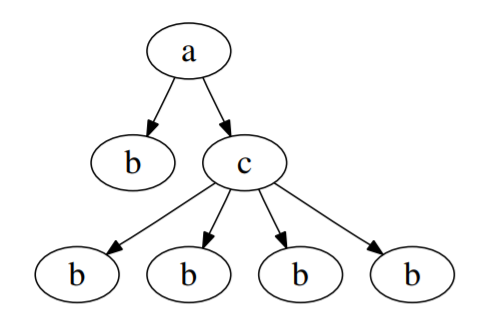
\includegraphics[width=0.3\textwidth]{ResearchNotes/rndhpc_not_dbg_2021_11_10/graph.png}
	\caption{Граф вызовов} 
\end{figure}

Узлами являются сами методы, а гранями -- их вызовы. Метод main() программы обычно является ее корнем, а все методы, вызываемые напрямую, являются ее дочерними элементами.

\textit{Редукция графа}

Трассировка представляется в виде графов вызовов, затем повторяющиеся вызовы методов, вызванные итерациями, удаляются, вместо этого вводятся веса ребер, представляющие частоту вызовов. 

\begin{figure}[!ht]
	\centering
	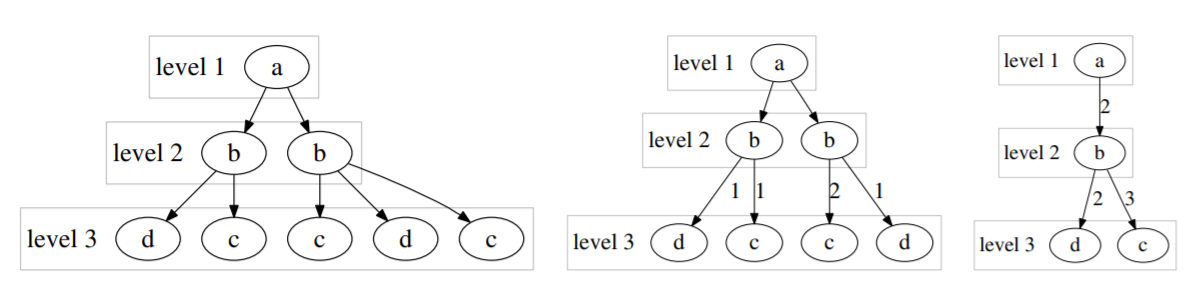
\includegraphics[width=1\textwidth]{ResearchNotes/rndhpc_not_dbg_2021_11_10/reduction.png}
	\caption{Редукция графа вызовов} 
\end{figure}

\textit{Поиск подграфов}

Для поиска подграфов используется фреймворк для ранжирования потенциально ошибочных методов.

После сокращения графов вызовов, полученных от правильного и неудачного выполнения программ, применяется поиск часто встречающихся замкнутых подграфов SG в наборе данных графа G, используя алгоритм CloseGraph. Полученный набор подграфов разделяется на те, которые встречаются при правильном и неудачном выполнении (SGcf), и те, которые возникают только при неудачном выполнении (SGf).

\textit{Анализ}

Два набора подграфов рассматриваются отдельно.

SGcf используется для построения рейтинга на основе различий в весах ребер при правильном и неудачном выполнении. Графы анализируются: применяется алгоритм выбора характеристик на основе энтропии к весам различных ребер для вычисления вероятности вызова метода и вероятности содержания в нем ошибки.

Алгоритм на основе энтропии не может обнаружить ошибки, которые не влияют на частоту вызовов и не учитывает подграфы, которые появляются только в ошибочной версии (SGf).

Поэтому отдельно рассчитывается оценка для методов, содержащихся только в ошибочной версии. Эта оценка - еще одна вероятность наличия ошибки, основанная на частоте вызовов методов при неудачных выполнениях.

Затем вычисляется общая вероятность наличия ошибки для каждого метода. Этот рейтинг дается разработчику программного обеспечения, который выполняет анализ кода подозрительных методов.

% --------------------------------------
\subsubsection{Интегрированная отладка моделей Modelica}

Далее представлен материал, являющийся результатом анализа работы \cite{Pop2014}.

Modelica -- объектно-ориентированный, декларативный язык моделирования сложных систем (в частности, систем, содержащих механические, электрические, электронные, гидравлические, тепловые, энергетические компоненты). 

\paragraph{Проблема}

Из за высокого уровня абстракции и оптимизации компиляторов, обеспечивающих простоту использования, ошибки программирования и моделирования часто трудно обнаружить.

\paragraph{Предложенное решение}

В статье представлена интегрированная среда отладки, сочетающая классическую отладку и специальные техники (для языков основанных на уравнениях) частично основанные на визуализации графов зависимостей.

\paragraph{Описание решения}

На этапе моделирования пользователь обнаруживает ошибку в нанесенных на график результатах, или код моделирования во время выполнения вызывает ошибку.

Отладчик строит интерактивный граф зависимостей (IDG) по отношению к переменной или выражению с неправильным значением.

Узлы в графе состоят из всех уравнений, функций, определений значений параметров и входных данных, которые использовались для вычисления неправильного значения переменной, начиная с известных значений состояний, параметров и времени.

Переменная с ошибочным значением (или которая вообще не может быть вычислена) отображается в корне графа.

Ребра могут быть следующих двух типов.
\begin{itemize}
	\item Ребра зависимости данных: направленные ребра, помеченные переменными или параметрами, которые являются входными данными (используются для вычислений в этом уравнении) или выходными данными (вычисляются из этого уравнения) уравнения, отображаемого в узле.
	\item Исходные ребра: неориентированные ребра, которые связывают узел уравнения с реальной моделью, к которой принадлежит это уравнение.
	ребра, указывающие из сгенерированного исполняемого кода моделирования на исходные уравнения или части уравнений, участвующие в этом коде \messnote{Непонятно}
\end{itemize}

Пользователь может:
\begin{itemize}
	\item Отобразить результаты симуляции, выбрав имя переменной или параметра(названия ребер). График переменной покажется в дополнительном окне. Пользователь может быстро увидеть, имеет ли переменная ошибочное значение.
	\item Отобразить код модели следуя по исходным ребрам.
	\item Вызвать подсистему отладки алгоритмического кода, если пользователь подозревает, что результат переменной, вычисленной в уравнении, содержащем вызов функции, неверен, но уравнение кажется правильным.
\end{itemize}

Используя эти средства интерактивного графа зависимостей, пользователь может проследить за ошибкой от ее проявления до ее источника.

%-------------------------------------------
\subsubsection{Систематические методы отладки для масштабных вычислительных фреймворков высокопроизводительных вычислений}

Далее представлен материал, являющийся результатом анализа работы \cite{Humphrey2014}.

Параллельные вычислительные фреймворки для высокопроизводительных вычислений играют центральную роль в развитии исследований, основанных на моделировании, в науке и технике.

Фреймворк Uintah был создан для решения сложных задач взаимодействия жидких структур с использованием параллельных вычислительных систем.

\paragraph{Проблема}

Поиск и исправление ошибок в параллельных фреймворках, возникающих из-за параллельного характера кода.

\paragraph{Предложенное решение}

В статье описывается подход к отладке крупномасштабных параллельных систем, основанный на различиях в исполнении между рабочими и нерабочими версиями. Подход основывается на трассировке стека вызовов.

Исследование проводилось для вычислительной платформы Uintah Computational Framework.

\paragraph{Описание решения}

Так как количество трассировок стека, которые можно получить при выполнении программы, может быть большим, для лучшего понимания используются графы, которые могут сжать несколько миллионов трассировок стека в одну управляемую фигуру. Метод основан на получении объединенных графов трассировки стека (CSTG). 

Хотя сбор и анализ трассировки стека ранее изучались в контексте инструментов и подходов, их внимание не было сосредоточено на кросс-версии (дельта) отладке.

\begin{figure}[!ht]
	\centering
	\begin{minipage}{0.45\textwidth}
	\centering
	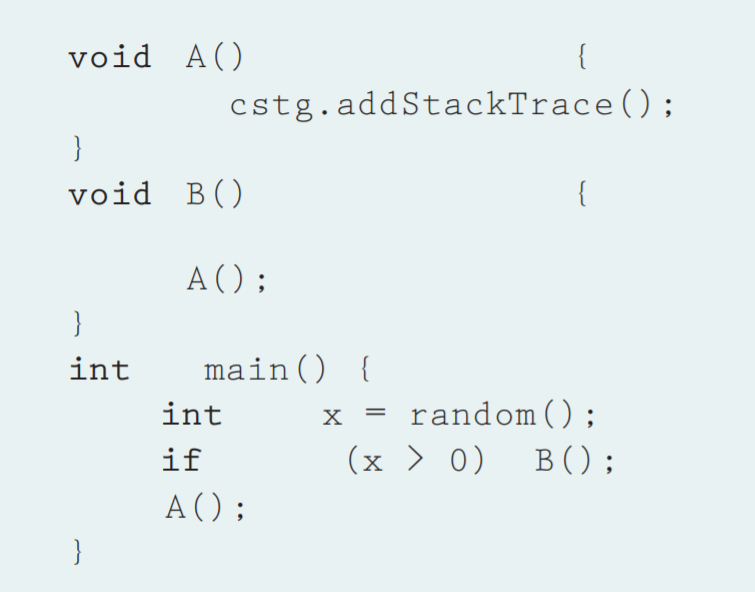
\includegraphics[width=1\textwidth]{ResearchNotes/rndhpc_not_dbg_2021_11_10/prog_ex.png}
	\end{minipage}
	\begin{minipage}{0.5\textwidth}
	\centering
	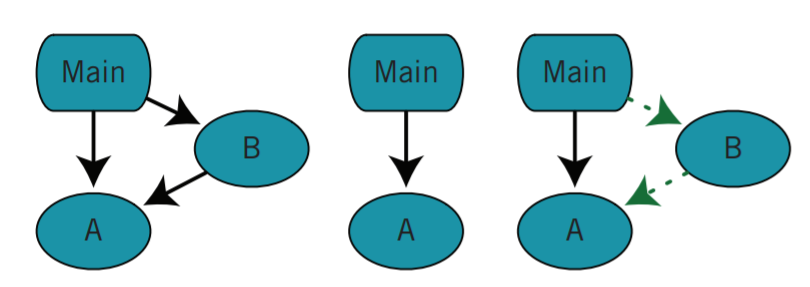
\includegraphics[width=1\textwidth]{ResearchNotes/rndhpc_not_dbg_2021_11_10/cstg.png}
	\end{minipage}
	\caption{Пример построения CSTG} 
\end{figure}

CSTG не записывают каждую активацию функции, а только те, что в трассировках стека ведут к интересующей функции (функциям), выбранной пользователем. Каждый узел CSTG представляет все активации конкретного вызова функции. Помимо имен функций, узлы CSTG также помечаются уникальными идентификаторами вызова. Грани представляют собой вызовы между функциями. 

\begin{figure}[!ht]
	\centering
	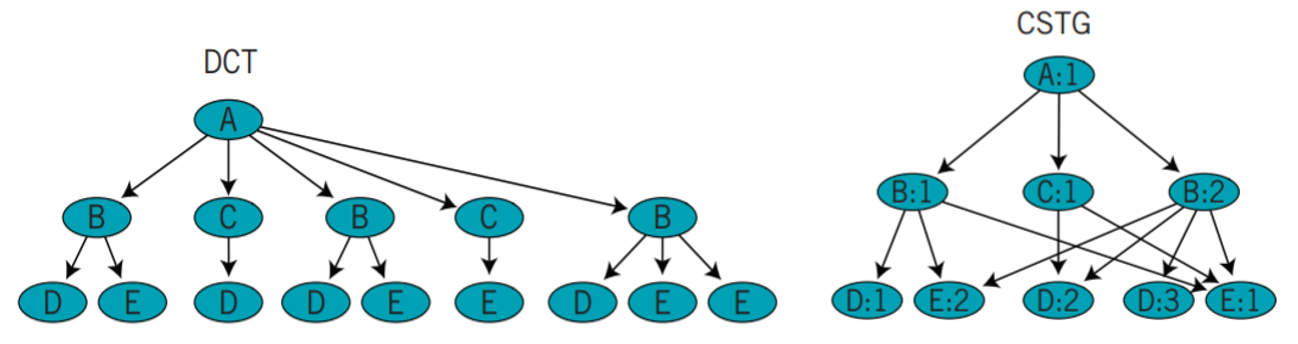
\includegraphics[width=1\textwidth]{ResearchNotes/rndhpc_not_dbg_2021_11_10/cstg2.png}
	\caption{CSTG} 
\end{figure}

Пользователю необходимо вставить в интересующие функции вызовы cstg.addStackTrace(). Инструмент CSTG автоматически запускает тестируемый пример с использованием различных сценариев, создает графы и помогает пользователям увидеть существенные различия между сценариями. Сама ошибка обычно обнаруживается и подтверждается с помощью традиционного отладчика, при этом дельта-группы CSTG наводят на место возникновения ошибки.

%----------------------------
\subsubsection{Ориентированный на данные фреймворк для отладки параллельных приложений}

Далее представлен материал, являющийся результатом анализа работы \cite{Dinh2013}.

\paragraph{Проблема}

Обнаружение ошибок в крупномасштабных научных приложениях, работающих на сотнях тысяч вычислительных ядер.

Неэффективность параллельных отладчиков для отладки пета-масштабных приложений.

\paragraph{Предложенное решение}

В этом исследовании представлена реализация фреймворка для отладки, ориентированного на данные, в котором в качестве основы используются утверждения. Подход, ориентированный на данные можно использовать для повышения производительности параллельных отладчиков. 

Метод, представленный в статье основан на параллельном отладчике Guard, который поддерживает тип утверждения во время отладки, называемые сравнительные утверждения. 

\paragraph{Описание решения}

Утверждение -- это утверждение о предполагаемом поведении компонента системы, которое должно быть проверено во время выполнения. В программировании программист определяет утверждение, чтобы гарантировать определенное состояние программы во время выполнения.

Пользователь делает заявления о содержимом структур данных, затем отладчик проверяет достоверность этих утверждений.

В следующем списке показаны примеры утверждений, которые можно использовать для обнаружения ошибок во время выполнения:

\begin{itemize}
	\item «Содержимое этого массива всегда должно быть положительным».
	\item «Сумма содержимого этого массива всегда должна быть меньше постоянной границы».
	\item «Значение в этом скаляре всегда должно быть больше, чем значение в другом скаляре».
	\item «Содержимое этого массива всегда должно быть таким же, как содержимое другого массива». 
\end{itemize}

В работе используются два новых шаблона утверждений помимо сравнительных: общие специальные утверждения и статистические утверждения.

\textit{Общие специальные} утверждения позволяют использовать простые арифметические и булевы операции.

\begin{figure}[!ht]
	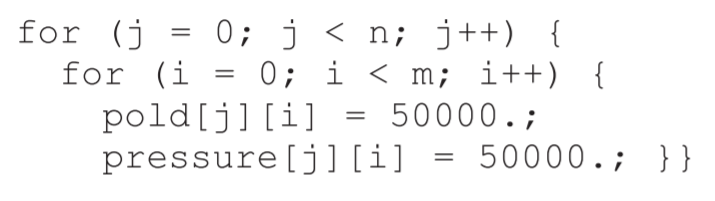
\includegraphics[width=0.5\textwidth]{ResearchNotes/rndhpc_not_dbg_2021_11_10/data_prog.png}
\end{figure}

Например, учитывая следующий фрагмент кода из исходного файла \textsf{init.c} и предполагая, что код вызывается с набором процессов \$a, можно рассмотреть следующее утверждение:

\begin{figure}[!ht]
	
\includegraphics[width=0.6\textwidth]{ResearchNotes/rndhpc_not_dbg_2021_11_10/assert1.png}
\end{figure}

Это утверждение гарантирует, что каждый элемент в структуре данных набора процессов \$a равен 50 000 в строке 180 исходного файла \textsf{init.c}.

Соответственно, \textit{сравнительные утверждения} позволяют сравнивать две отдельные структуры данных во время выполнения.

Следующее утверждение сравнивает данные из big_var в \$a в строке 4300 исходного файла ref.c с large_var в \$b в строке 4300 исходного файла \textsf{sus.c}.

\begin{figure}[!ht]
	
\includegraphics[width=0.8\textwidth]{ResearchNotes/rndhpc_not_dbg_2021_11_10/assert2.png}
\end{figure}

\textit{Статистические утверждения} - это определяемый пользователем предикаты, состоящие из двух моделей данных в форме либо статистических примитивов (средние значения, значения стандартного отклонения), либо функциональных моделей (гистограммы, функции плотности)

Статистические утверждения позволяют пользователю сравнивать информацию о шаблонах данных между двумя структурами данных, тогда как более ранние утверждения требовали сравнения точных значений.

Например, можно утверждать, что среднее значение большого набора данных находится между определенными границами до или после вызова функции или что количество элементов в массиве должно находиться в определенном диапазоне.

%-------------------------
\subsubsection{Определение степени и источников недетерминизма в приложениях MPI с помощью ядер графов}

Далее представлен материал, являющийся результатом анализа работы \cite{Chapp2021}.

\paragraph{Проблема}

Выявление причин сбоев воспроизводимости в приложениях на экзафлопсных платформах.

Крупномасштабные приложения MPI обычно принимают гибкие решения во время выполнения том порядке, в котором процессы обмениваются данными, чтобы улучшить свою производительность. Следовательно, недетерминированные коммуникативные модели стали особенностью этих научных приложений в системах высокопроизводительных вычислений.

Недетерминизм мешает разработчикам отслеживать вариации выполнения программы для отладки. Также сложно воспроизвести результаты при повторных запусках, что затрудняет доверие к научным результатам.

\paragraph{Предложенное решение}

Фреймворк для определения источников недетерминизма с использованием графов событий. 

\paragraph{Описание решения}

Параллельное выполнение программы моделируется в виде ориентированных графов событий, ядра графов используются, чтобы охарактеризовать изменения межпроцессного взаимодействия от запуска к запуску. Ядра могут количественно определять тип и степень недетерминизма, присутствующего в моделях коммуникации MPI.

Фреймворк позволяет найти первопричины недетерминизма в исходном коде без знания коммуникативных паттернов приложения.

Платформа моделирует недетерминизм в следующие три этапа. 

\paragraph{Этап первый. Сбор трассировки выполнения.} Фреймворк фиксирует трассировку нескольких выполнений недетерминированного приложения с помощью двух модулей трассировки: CSMPI (фиксирует стек вызововов, связанных с вызовами функций MPI) и DUMPI (фиксирует порядок отправляемых и получаемых сообщений для каждого процесса MPI).

Для каждого выполнения приложения фреймворк генерирует один файл трассировки CSMPI и один файл трассировки DUMPI для каждого процесса MPI (или ранга). Файлы трассировки впоследствии загружаются конструктором графа событий для восстановления порядка сообщений выполнения.

\paragraph{Этап второй. Построение модели графа событий.} На втором этапе фреймворк моделирует выполнение недетерминированного приложения в виде ориентированного ациклического графа (DAG), используя файлы трассировки, созданные на первом этапе.

Здесь вершины представляют собой связи point-to-point, такие как отправка и получение сообщения, а направленные ребра представляют отношения между этими событиями. Модели межпроцессного взаимодействия этой формы обычно называются графами событий.

\begin{figure}[!ht]
	\centering
	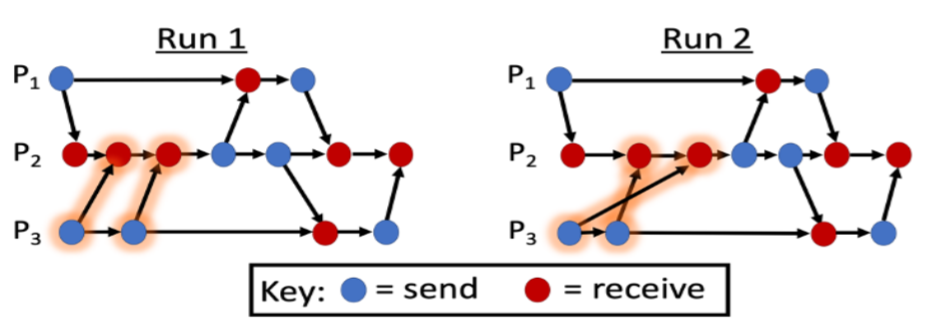
\includegraphics[width=0.7\textwidth]{ResearchNotes/rndhpc_not_dbg_2021_11_10/dga.png}
	\caption{DGA} 
\end{figure}

Затем используются ядра графов для количественной оценки (несходства) графов событий, тем самым количественно оценивая степень проявления недетерминированности в приложении.

Ядра графов представляют собой семейство методов для измерения структурного сходства графов. 

Простыми словами, ядро графа можно рассматривать как функцию, которая подсчитывает совпадающие подструктуры (например, поддеревья) двух входных графов, как показано на рис.~\ref{lab.rndhpc2021.11.10.010}, сопоставляя пары графов со скалярами, которые количественно определяют, насколько они похожи.

\begin{figure}[!ht]
	\centering
	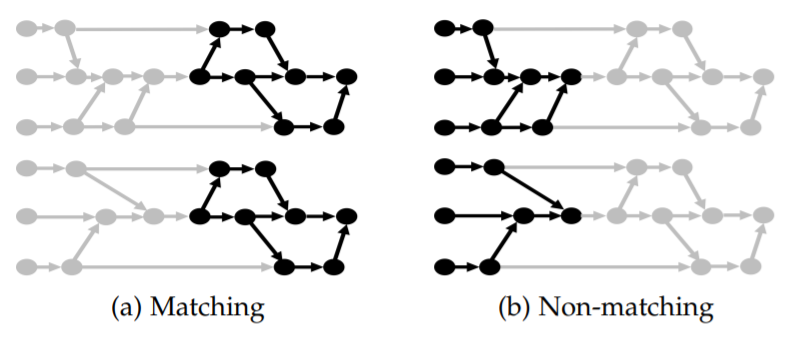
\includegraphics[width=0.6\textwidth]{ResearchNotes/rndhpc_not_dbg_2021_11_10/graph_comp.png}
	\caption{Сравнение двух графов}\label{lab.rndhpc2021.11.10.010}
\end{figure}

\paragraph{Этап третий. Анализ графа событий.} На последнем этапе анализ графа событий позволяет ученым количественно оценить недетерминированность многократного выполнения приложения MPI без каких-либо знаний о коммуникативных моделях приложения MPI.

%----------------------------------------------------------
% Атрибуты задачи
\noteattributes{}
%----------------------------------------------------------


%----------------------------------------------------------
\def\notedate{2021.11.22}
\def\currentauthor{Крехтунова Д.Д. (РК6-73Б)}
%----------------------------------------------------------
\notestatement{rndhpcdbg}{Web-инструменты для древовидного представления ассоциативных массивов, визуализация ассоциативных массивов (первичный обзор литературы)}

%---------------------------------------------------------
\subsubsection{Ассоциативные массивы}

Ассоциативный массив -- это массив, в котором обращение к значению осуществляется по ключу (того или иного типа).

Часто в качестве ключа используется не индекс, а строка, задаваемая программистом. Таким образом представить ассоциативный массив можно как набор пар ``ключ-значение''. При этом каждое значение связано с определённым ключом.

Поддержка ассоциативных массивов есть во многих интерпретируемых языках программирования высокого уровня, таких, как Perl, PHP, Python, Ruby, Tcl, JavaScript и других.

\paragraph{Реализации ассоциативного массива} Простейший способ хранения ассоциативных массивов -- список пар (ключ, значение), где \textit{ключ} определяет ``индекс'' элемента, а \textit{значение} -- значение элемента с этим индексом.

Наиболее популярными являются реализации ассоциативных массивов, основанные на различных деревьях поиска. Так, например, в стандартной библиотеке STL языка C++ контейнер \textsl{map<K,T>} реализован на основе красно-чёрного дерева \cite{XXX}. В языках Java, Ruby, Tcl, Python используется один из вариантов хеш-таблицы \cite{YYY}.\messnote{Какой именно один из?} Известны и другие реализации (aaa, ммм, ...).\messnote{Какие именно ?}

Операции с деревом работают быстрее. При реализации на основе списков все функции требуют $O(n)$ операций, где $n$ -- количество элементов в рассматриваемой структуре. Операции над деревьями же требуют $O(h)$, где $h$ -- максимальная глубина дерева.\messnote{При переводе к n получается O(n logn). Следует писать так, чтобы было ясно в чём приемущество.}

Данные в дереве хранятся в его вершинах. В программах вершины дерева обычно представляют структурой, хранящей данные и две ссылки на левого и правого сына. 

\begin{figure}[!ht]
	\centering
	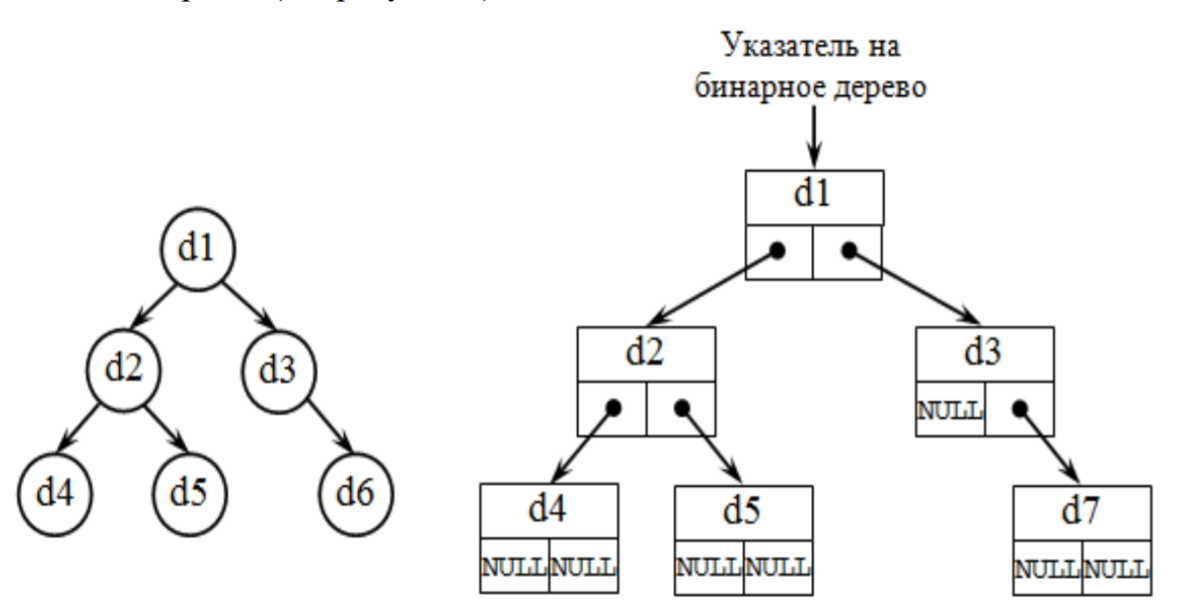
\includegraphics[width=0.6\textwidth]{ResearchNotes/rndhpc_not_dbg_2021_11_22/bin_tree.png}
	\caption{Пример представления бинарного дерева} 
\end{figure}

%---------------------------------------------------------
\subsubsection{Набор библиотек TnT для web-визуализации деревьев и аннотаций на основе трассировок}

В статье \cite{Pignatelli2016} представлен набор библиотек, предназначенных для web-визуализации деревьев и трассировок.

В статье говорится в первую очередь о визуализации биологических данных в веб-приложениях. Но представленные библиотеки не имеют узкой направленности и могут использоваться для разных целей.

Библиотеки TnT (англ.~Trees and Tracks) предназначены для создания настраиваемых, динамических и интерактивных визуализаций деревьев и аннотаций на основе треков. 

Библиотеки написаны на Javascript с использованием библиотеки D3, которая сама по себе является мощным инструментом визуализации данных. Она использует стандарты масштабируемой векторной графики (SVG), HTML и CSS.

Ниже приведено краткое описание библиотек TnT, непосредственно связанных с визуализацией деревьев.

\begin{itemize}
	\item \textit{TnT Tree}
	
	Эта библиотека построена на основе кластерного расположения D3 (D3 cluster layout) и позволяет создавать динамические и интерактивные деревья. Он состоит из нескольких настраиваемых элементов: макета, определяющего общую форму дерева, узлов дерева в которых можно изменять форму, размер и цвет, ярлыков, состоящих из текста или изображений и данных для загрузки объектов Javascript или строк newick / nhx.2.2 TnT Tree Node.
	
	PhyloCanvas - аналогичный проект, предлагающий средства для визуализации деревьев. В качестве основной технологии в нем используется Canvas. Но библиотеки TnT более универсальны и поддерживают интеграцию с другими библиотеками. Документацию и примеры для TnT Tree можно найти по ссылке http://tntvis.github.io/tnt.tree/.
	
	\item \textit{TnT Tree Node}	
	
	Эта библиотека предоставляет методы для управления деревом на уровне данных и используется TnT Tree, хотя также может использоваться и независимо. Методы, включенные в TnT Tree Node, варьируются от вычисления наименьшего общего предка набора узлов до извлечения поддеревьев. Документацию для этой библиотеки можно найти как часть документации библиотеки TnT Tree.
\end{itemize}

%---------------------------------------------------------
\subsubsection{Программное обеспечение Empress интерактивного и исследовательского анализа многомерных наборов данных на основе деревьев}

В работе \cite{Cantrell2021} представлен интерактивный web-инструмент EMPress для визуализации деревьев в контексте микробиома, метаболома и других областей. EMPress предоставляет широкие функциональные возможности, такие как анимация объектов, наряду со стандартными функциями визуализации дерева.

EMPress реализован в виде подключаемого модуля QIIME 2 (или отдельной программы Python, которую можно использовать вне QIIME 2), способной создавать HTML-документы с автономным пользовательским интерфейсом визуализации. Кодовая база состоит из компонента Python и компонента JavaScript. Кодовая база Python отвечает за проверку данных, предварительную обработку, фильтрацию и форматирование. Взаимодействие с пользователем, рендеринг и генерация рисунков обрабатываются базой кода JavaScript. 

Кодовая база Python EMPress использует такие модули, как NumPy, SciPy, Pandas, Click, Jinja2, scikit-bio, формат BIOM и EMPeror. 

В кодовой базе JavaScript используются Chroma.js, FileSaver.js, glMatrix, jQuery, Require.js, Spectrum, и Underscore.js. 

%---------------------------------------------------------
\subsubsection{Программный инструмент Treemap визуализации иерархических структур}

В статье \cite{Jadeja2020} представлена интерактивная версия Treemap.

В теории графов дерево -- это особый тип графа, который связан и ацикличен~\cite{ZZZ}. Обычно деревья представляются визуально с помощью диаграмм узлов и связей (древовидных диаграмм). В деревьях ребра присутствуют только между соседними слоями, и, следовательно, деревья наилучшим образом подходят для представления иерархических данных, для которых характерно расположение элементов на различных уровнях относительно друг друга: ``ниже'', ``выше'' или ``на одном уровне''.

Treemap - это метод визуализации иерархических структур. Используя этот метод, можно отобразить дерево с миллионами узлов в ограниченном пространстве. Основная идея, лежащая в основе этого метода визуализации, состоит в том, чтобы выделиять прямоугольники для родительских узлов, а для дочерних узлов блоки (прямоугольники) в соответствующем родительском прямоугольнике. 

Интерфейс создавался с использованием html / css с jQuery для обработки событий, связанных с кликами.Входными данными для интерфейса является дерево родительских указателей (parent pointer tree - структура данных N-арного дерева, в которой каждый узел имеет указатель на свой родительский узел, но не указывает на дочерние узлы). 

%---------------------------------------------------------
\subsubsection{Web-инструмент DoubleRecViz для визуализации согласования деревьев транскриптов и генов}

В статье \cite{Kuitche2021} представлен веб-инструмент для визуализации согласований между филогенетическими деревьями (деревья, отражающее эволюционные взаимосвязи между различными видами, имеющими общего предка).

В статье описан формат DoubleRecViz, основанный на формате phyloXML (XML, предназначенный для описания филогенетических деревьев и связанных с ними данных). 

DoubleRecViz написан на Python и использует библиотеку Dash, которая предоставляет функции динамической визуализации веб-данных.
Dash является связкой Flask, React.Js, HTML и CSS.

Приложения на Dash — веб-серверы, которые запускают Flask и связывают пакеты JSON через HTTP-запросы. Интерфейс Dash формирует компоненты, используя React.js.

Компоненты Dash — это классы Python, которые кодируют свойства и значения конкретного компонента React и упорядочиваются как JSON. 

Полный набор HTML-тегов также обрабатывается с помощью React, а их классы Python доступны через библиотеку. CSS и стили по умолчанию хранятся вне базовой библиотеки, чтобы сохранить принцип модульности и независимого управления версиями.

%----------------------------------------------------------
% Атрибуты задачи
\noteattributes{}
%----------------------------------------------------------


%----------------------------------------------------------
\def\notedate{2021.12.19}
\def\currentauthor{Крехтунова Д.Д. (РК6-73Б)}
%----------------------------------------------------------
\notestatement{rndhpcdbg}{Постановка задачи}

%---------------------------------------------------------
\subsubsection{Концептуальная постановка задачи}\

Разработка web-ориентированного отладчика для отслеживания текущих значений элементов данных в узлах графовой модели реализации вычислительного метода.

Реализация отладчика поможет отслеживать текущие значения отдельных элементов данных в узле графа, что упростит процесс разработки графоориентированных решателей. 
\newline

\textbf{Объект разработки}: графовая модель вычислительного метода, представленная ориентированными графами с формализуемым назначением узлов и рёбер.

\textbf{Цель разработки}: Создание программного web-инструментария для визуализации данных в произвольном состоянии данных (узле) при проведении текущего расчета.

\textbf{Задачи} курсового проекта:
\begin{enumerate}
	\item Провести обзор литературы по теме: «Автоматические методы отладки наукоемкого кода».
	\item Определить возможные типы элементов данных графовой модели и реализовать методы визуализации для каждого из них.
	\item Разработать функцию, позволяющую определить тип данных, хранящихся в ассоциативном массиве (хранение данных осуществляется в объекте типа dict). 
	\item Визуализировать данные в виде древовидной структуры.
\end{enumerate}


%----------------------------------------------------------
% Атрибуты задачи
\noteattributes{}
%----------------------------------------------------------



%----------------------------------------------------------
\section{\rndprojectdscr{rndhpcedt}}

%----------------------------------------------------------
\def\notedate{2021.10.05}
\def\currentauthor{Ершов В. (РК6-72Б)}
%----------------------------------------------------------
\notestatement{rndhpcedt}{Обзор языка описания графов DOT}

Язык описания графов DOT предоставляется пакетом утилит Graphviz (Graph Visualization Software). Пакет состоит из набора утилит командной строки и программ с графическим интерфейсом, способных обрабатывать файлы на языке DOT, а также из виджетов и библиотек, облегчающих создание графов и программ для построения графов. Более подробно будет рассмотрена утилита dot.
\newline\newline
dot - инструмент для создания многоуровневого графа с возможностью вывода изображения полученного графа в различных форматах (PNG, PDF, PostScript, SVG и др.).
\newline\newline
Установка graphviz

\quad Linux: \lstinline$sudo apt install graphviz$

\quad MacOS: \lstinline$brew install graphviz$
\newline\newline
Вызов всех программ Graphviz осуществляется через командную строку, в процессе ознакомления с языком использовалась следующая команда

\quad\lstinline$dot -Tpng <pathToDotFile> -o <imageName>$
\newline
В результате выполнения этой команды будет создано изображение графа в формате png
\newline\newline
Пример описания простого графа\newline\newline
\begin{minipage}{0.2\textwidth}
		\begin{verbatim}
				digraph G {
				    a -> b;
				    a -> d -> c;
				    d -> e;
				}
		\end{verbatim}
	\end{minipage}
	\hfill
	\begin{minipage}{0.75\textwidth}
	 	{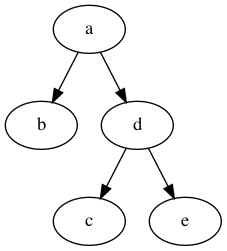
\includegraphics[width=0.3\textwidth]{ResearchNotes/images/image4.png}\xspace}
	\end{minipage}
\newline\newline\newline
Более подробная информация с примерами представлена в обзоре литературы, который находится по следующему пути:
\newline
01 - Курсовые проекты/2021-2022 - Разработка web-ориентированного редактора графовых моделей /0 - Обзор литературы/	

%----------------------------------------------------------
% Атрибуты задачи
\noteattributes{}
%----------------------------------------------------------
%----------------------------------------------------------
\def\notedate{2021.12.04}
\def\currentauthor{Ершов В. (РК6-72Б)}
%----------------------------------------------------------
\notestatement{rndhpcedt}{Краткое описание алгоритма визуализации графа}

В ходе разработки web-ориентированного редактора графов, который позволяет импортировать и экспортировать файлы в формате aDOT~\cite{SokADOT}, был разработан алгоритм визуализации графов. В этой заметке будет рассмотрен этот алгоритм и приведено несколько примеров aDOT файлов, которые корректно визуализируются, используя этот алгоритм.

Теоретические основы и назначение графоориентированной программной инженерии представлены в работе~\cite{SokPersh2018GBSE}. Принципы применения графоориентированного подхода зафиксированы в патенте~\cite{patentRU2681408}. 

Один из самых важных критериев построенного графа -- это его читаемость. Граф должен быть построен корректно и недопускать неоднозначностей при его чтении. Например, вершины не должны налегать друг на друга, ребра не должны пересекаться, создавая сложные для восприятия связи.

Проведя длительную аналитическую работу, было принято решение разбивать граф по уровням. Рассмотрим следующее aDOT-определение графовой модели \textsf{G} (листинг~\ref{lst:gm.exmpl.1}).

\begin{lstlisting}[frame=single, label={lst:gm.exmpl.1}, caption={Пример aDOT-определение простейшей графовой модели \textsf{G}}, language=aDOTExample]
digraph G {
// Parallelism
	s1 [parallelism=threading]
// Graph definition
	__BEGIN__ -> s1
	s4 -> s6 [morphism=edge_1]
	s5 -> s6 [morphism=edge_1]
	s1 => s2 [morphism=edge_1]
	s1 => s3 [morphism=edge_1]
	s2 -> s4 [morphism=edge_1]
	s3 -> s5 [morphism=edge_1]
	s6 -> __END__ 
}
\end{lstlisting}

Если нарисовать такой граф на бумаге, то становится очевидно, что каждый набор вершин имеет одну координату по оси X, а связанные с ними вершины находятся правее по координате X, таким образом напрашивается разбиение графа по уровням. На рисунке (\ref{fig:graph_levels}) представлен этот граф, разбитый на уровни.

\begin{figure}[ht!]
\center{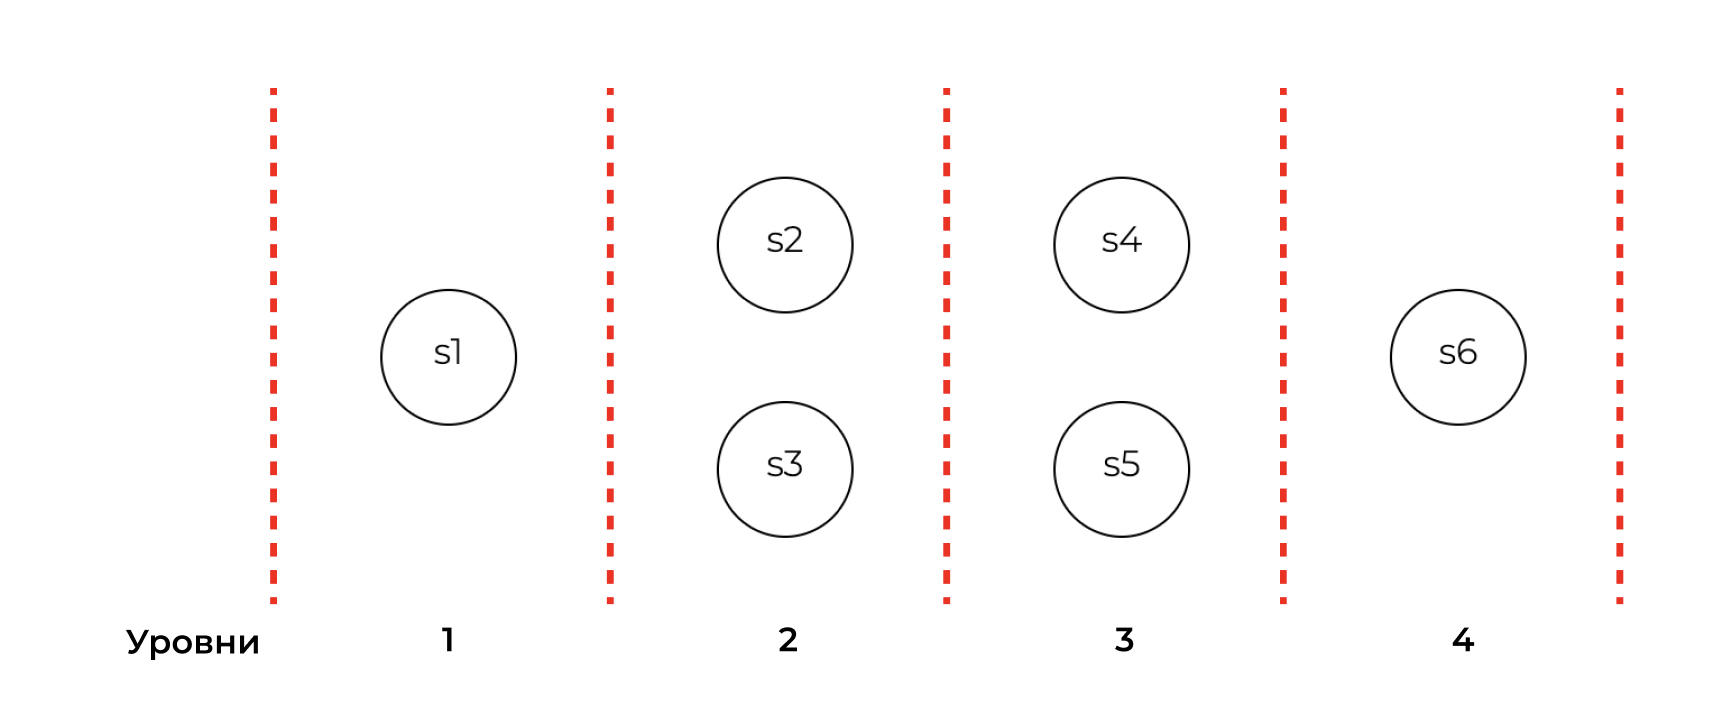
\includegraphics[width=0.8\linewidth]{ResearchNotes/images/graph_levels.png}}
\caption{Узлы графовой модели \textsf{G}, представленные на разных ``уровнях''}
\label{fig:graph_levels}
\end{figure}

Разбиение графа по уровням является основой алгоритма визуализации, далее на примере более сложного графа поэтапно разберем алгоритм.

Рассмотрим следующий файл на языке aDOT (листинг~\ref{lst:gm.exmpl.2}).

\begin{lstlisting}[frame=single, label={lst:gm.exmpl.2}, caption={Пример aDOT-определения графовой модели \textsf{TEST}}, language=aDOTExample]
digraph TEST
{
// Parallelism
	s11 [parallelism=threading]
	s4 [parallelism=threading]
	s12 [parallelism=threading]
	s15 [parallelism=threading]
	s2 [parallelism=threading]
	s8 [parallelism=threading]
// Functions
	f1 [module=DEFAULT_VALUE, entry_func=DEFAULT_VALUE]
// Predicates
	p1 [module=DEFAULT_VALUE, entry_func=DEFAULT_VALUE]
// Edges
	edge_1 [predicate=p1, function=f1]
// Graph model description
	__BEGIN__ -> s1
	s6 -> s8 [morphism=edge_1]
	s7 -> s8 [morphism=edge_1]
	s10 -> s8 [morphism=edge_1]
	s11 => s8 [morphism=edge_1]
	s11 => s9 [morphism=edge_1]
	s14 -> s9 [morphism=edge_1]
	s3 -> s9 [morphism=edge_1]
	s4 => s6 [morphism=edge_1]
	s4 => s7 [morphism=edge_1]
	s4 => s10 [morphism=edge_1]
	s4 => s11 [morphism=edge_1]
	s12 => s4 [morphism=edge_1]
	s12 => s14 [morphism=edge_1]
	s13 -> s3 [morphism=edge_1]
	s15 => s14 [morphism=edge_1]
	s15 => s14 [morphism=edge_1]
	s2 => s12 [morphism=edge_1]
	s2 => s13 [morphism=edge_1]
	s2 => s15 [morphism=edge_1]
	s1 -> s2 [morphism=edge_1]
	s8 => s9 [morphism=edge_1]
	s8 => s6 [morphism=edge_1]
	s9 -> __END__ 
}
\end{lstlisting}

В результате визуализации модели будет получен граф, представленный на рисунке (\ref{fig:main_graph}).

\begin{figure}[ht!]
\center{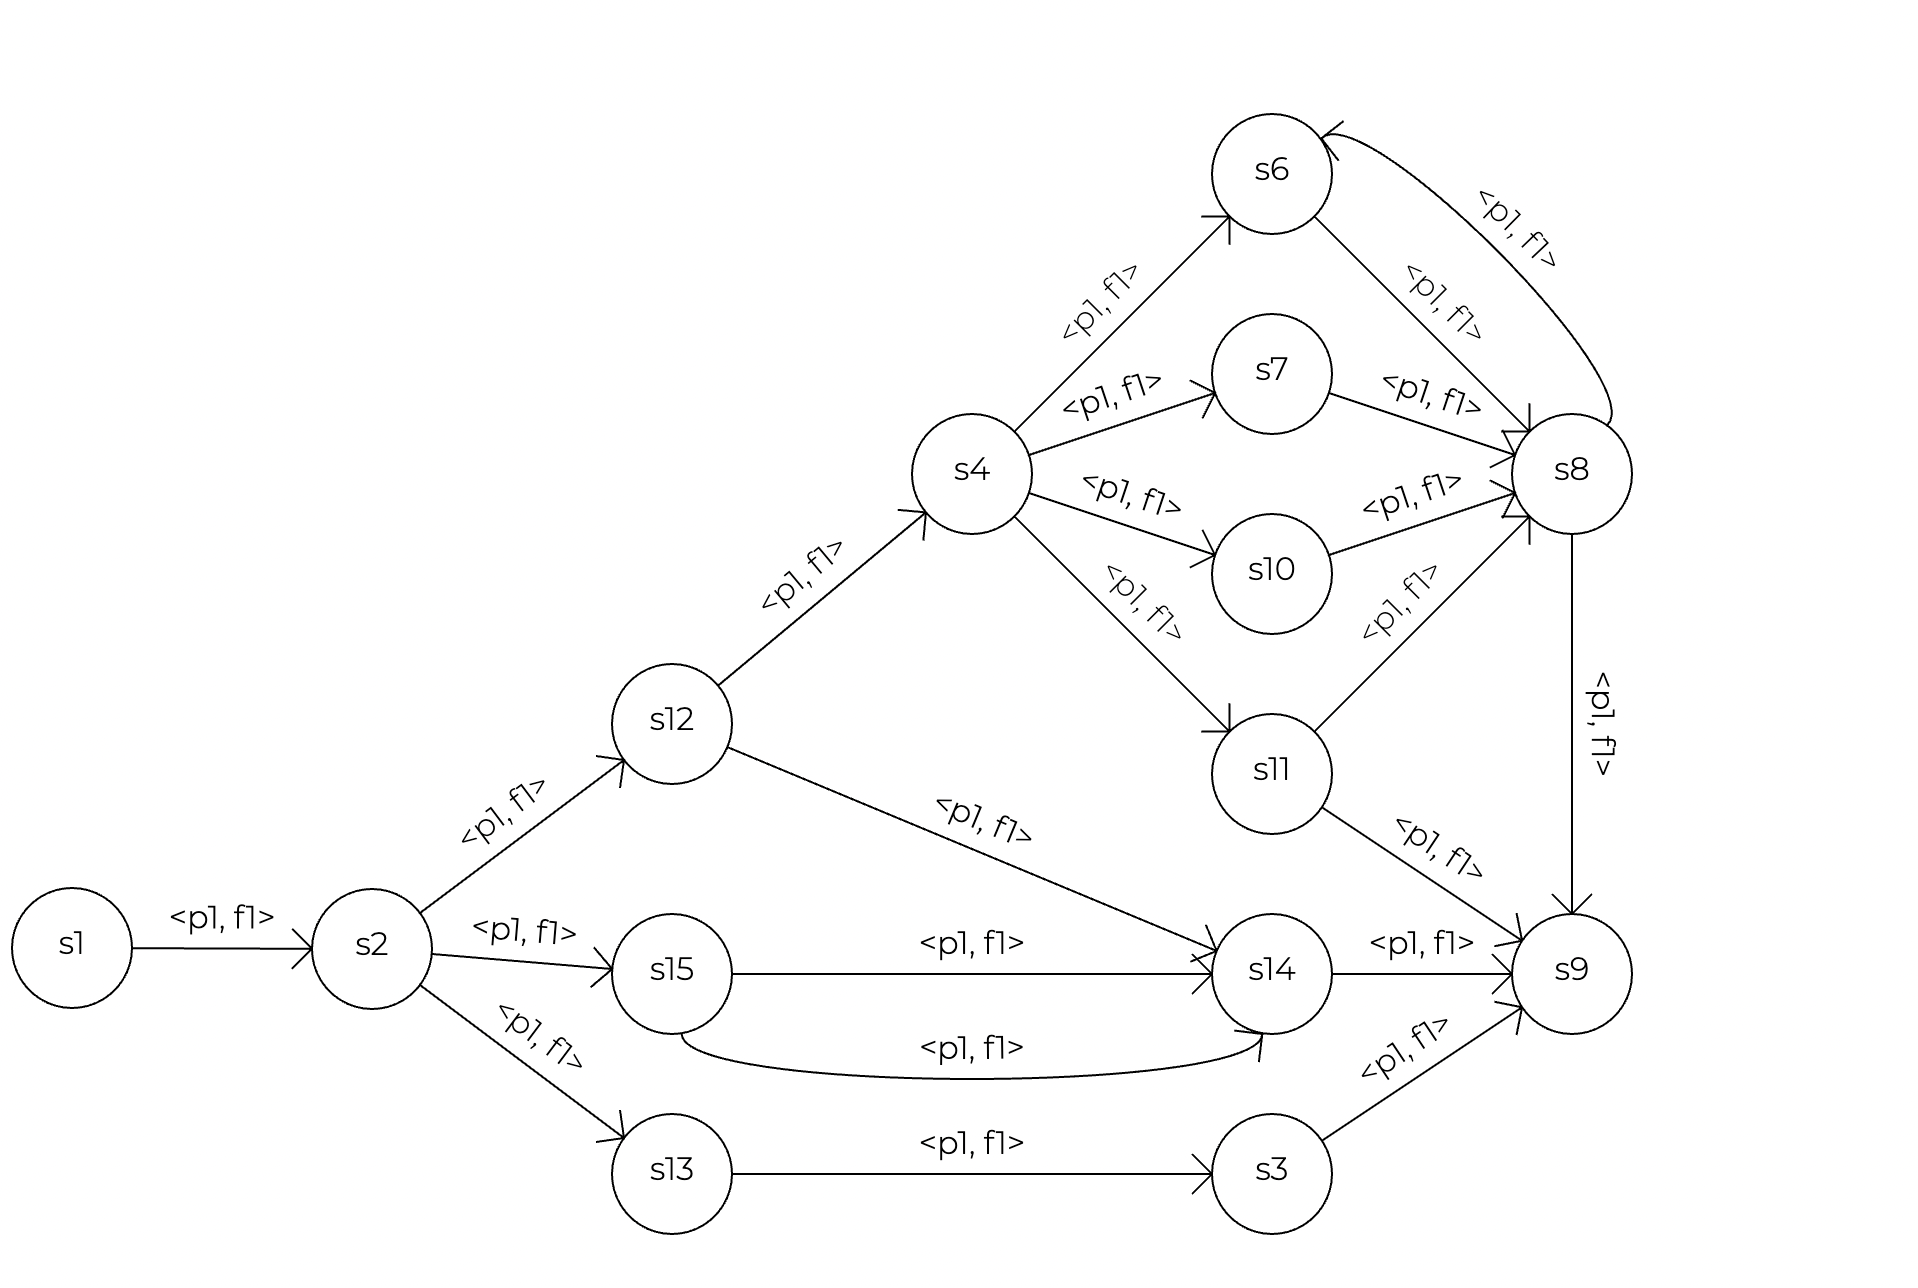
\includegraphics[width=0.85\linewidth]{ResearchNotes/images/main_graph.png}}
\caption{Визуализация графовой модели \textsf{TEST}}\label{fig:main_graph}
\end{figure}

Основная задача алгоритма -- это отрисовать вершины графа в корректных позициях, а затем построить между ними ребра. Поскольку редактор графов -- это web-ориентированное приложение, то вся бизнес-логика написана на языке \textsf{JavaScript}. В \textsf{JavaScript} имеется очень удобный инструмент -- объекты. Аналогами объектов в других языках программирования являются хэш-карты, но в Javascript возможности использования объектов гораздо шире. Всю информацию об уровнях графа будем хранить в объекте levels. Ниже представлено как выглядит объект levels для рассматриваемого выше графа:

\begin{verbatim}
{
	"1":[{"s1":[]}],
	"2":[{"s2":["s1"]}],
	"3":[{"s12":["s2"]}, {"s13":["s2"]}, {"s15":["s2"]}],
	"4":[{"s4":["s12"]}],
	"5":[{"s9":["s14","s3"]}, {"s6":["s4"]}, {"s7":["s4"]}, {"s10":["s4"]}, 
	{"s11":["s4"]},	{"s14":["s12","s15"]}, {"s3":["s13"]}],
	"6":[{"s8":["s6","s7","s10","s11"]}, {"s9":["s11","s14","s3"]}]
}
\end{verbatim}

Ключами объекта levels являются номера уровней, представленные в формате string. Свойсвами являются массивы, на один уровень - один массив. Каждый элемент массива содержит информацию об одной вершине на этом уровне, следовательно количество вершин на уровне - это размер массива. Далее заметим, что элемент массива это не просто string с названием вершины, а объект. Этот объект содержит один ключ - название вершины на этом уровне, а свойством является массив, который содержит список вершин из которых перешли в эту вершину (переход только по одному ребру).

В качестве примера рассмотрим уровень 5 объекта levels, который был представлен ранее.

\begin{minipage}{0.5\textwidth}
	\begin{verbatim}
	{
	  "5":[{"s9":["s14","s3"]}, {"s6":["s4"]}, {"s7":["s4"]}, 
	  {"s10":["s4"]}, {"s11":["s4"]}, {"s14":["s12","s15"]}, {"s3":["s13"]}],
	}
	\end{verbatim}
\end{minipage}


Уровень 5 в графе представлен 7-ю вершин: ``s9'', ``s6'', ``s7'', ``s10'', ``s11'', ``s14'', ``s3''. Например, в вершину ``s6'' мы пришли из вершины ``s4'', таким образом, по ключу ``s6'' находится массив c один элементом ``s4''
\begin{verbatim}
{"s6": ["s4"]}
\end{verbatim}

На рисунке (\ref{fig:main_graph_level5}) представлен граф с выделенным уровнем №5.

\begin{figure}[ht!]
\center{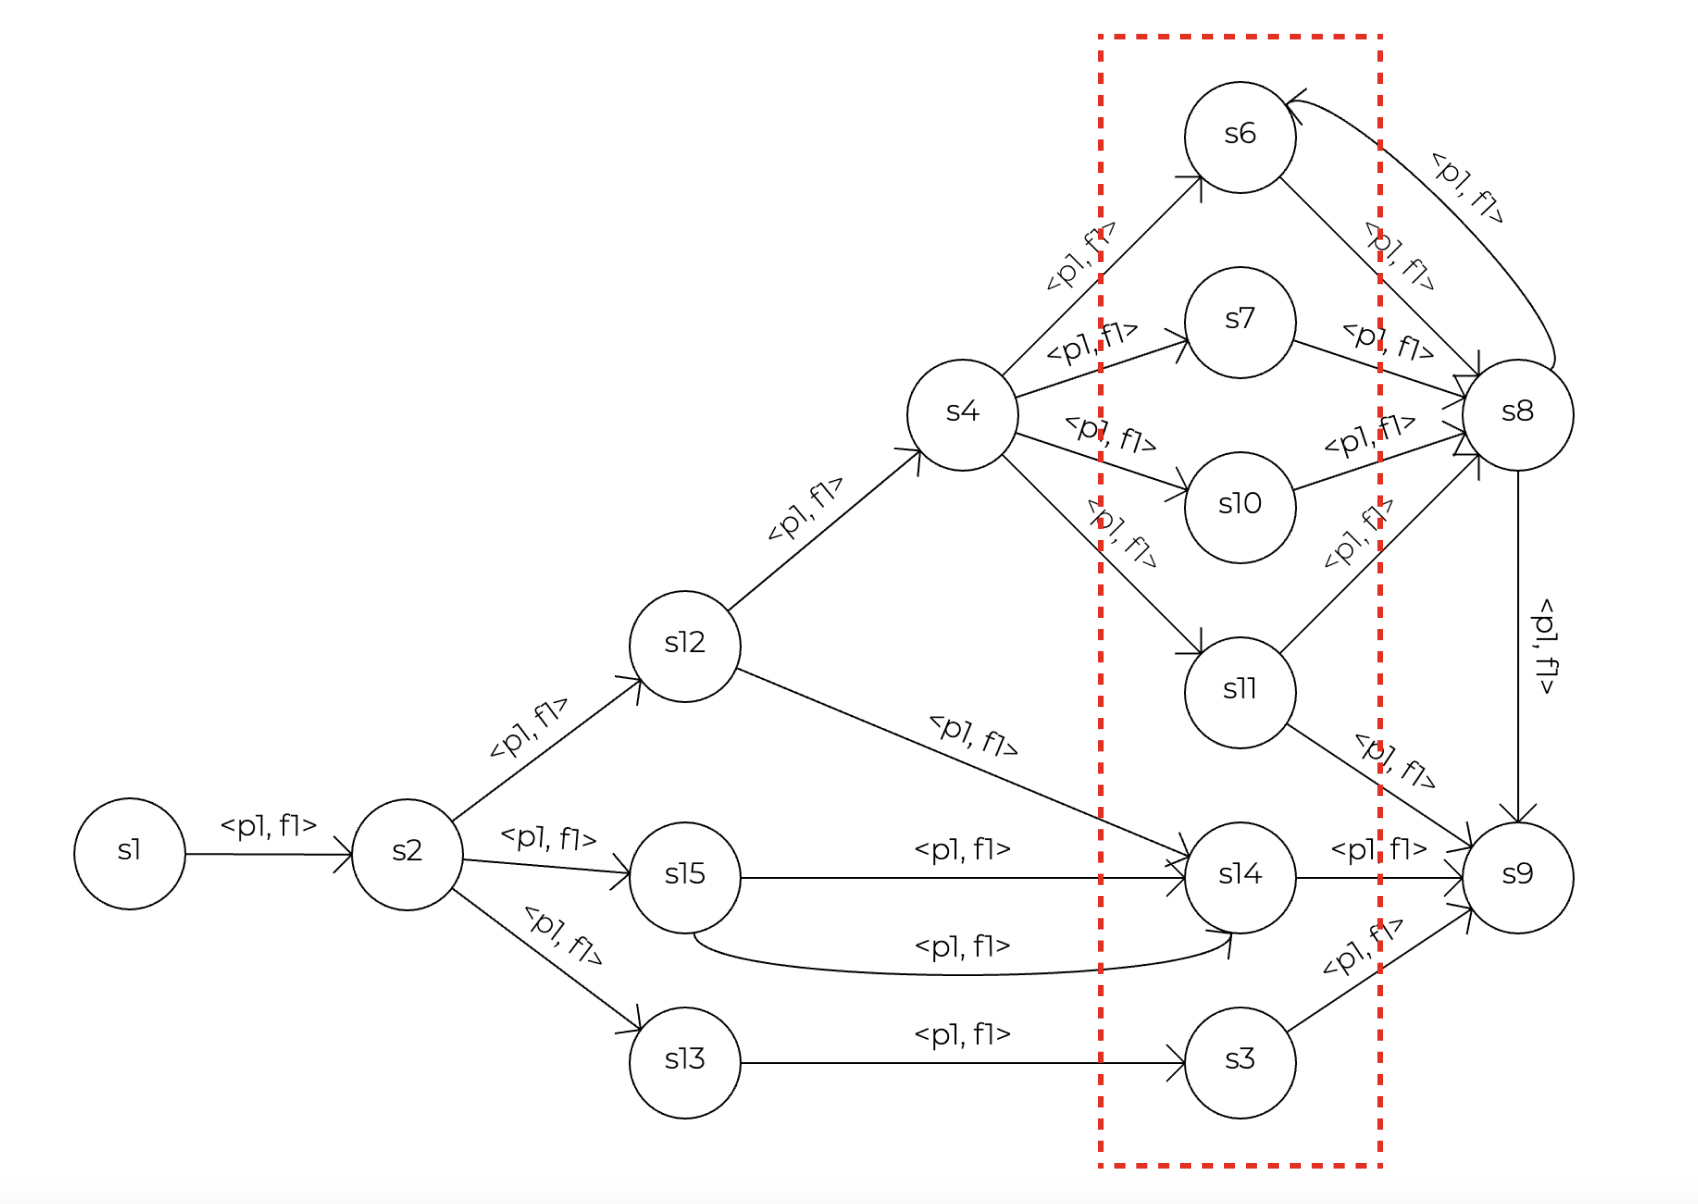
\includegraphics[width=0.85\linewidth]{ResearchNotes/images/main_graph_level5.png}}
\caption{Уровень №5 на графе}
\label{fig:main_graph_level5}
\end{figure}

Обратим вниманием на то, что в объекте levels для уровня №5 содержится вершина $s_9$ которой нет на уровне №5, а она присутствует только на уровне №6. Заполнение объекта levels происходит слево-направо, то есть от меньшего
уровня к большему, например, в графе представленном выше есть связь $s_{13} \rightarrow s_3$, таким образом пока в объект levels не будет записана вершина $s_{13}$, мы не сможем записать связанную с ней вершину $s_3$.

Обратным образом происходит дублирование вершин, если обратиться к описанию графовой модели предсталвенной выше, то можно заметить такую связь: $s_1 \rightarrow s_2 \rightarrow s_{13} \rightarrow s_3 \rightarrow s_9$. При начальной инициализации объекта levels $s_1$ будет находиться на уровне 1, $s_2$ будет находиться на уровне 2 и так далее. Таким образом, вершина $s_3$ будет находиться на уровне 4, что не совсем корректно. Обработка таких ситуаций является углублением в реализацию алгоритма и в этой заметке не будет подробно описываться.

Для разрешения подобных коллизий после начальной инициализации объекта levels ``в лоб'' предусмотрено множество дополнительных проверок. Таким образом, на выходе мы получаем корректно сформированный объект levels и дополнительно формируем объект, который будет хранить информацию о вершинах которые находятся не на своем уровне, эти вершины не будут отрисовываться, но при этом они будут учитываться при выравнивании связанных с ними вершин, следовательно просто удалить такие вершины из объекта levels нельзя.

Сама визуализация вершин после формирования объекта levels также является темой отдельной заметки. На данном этапе работы над проектом сначала строится уровень содержащий наибольшее количество вершин, затем строятся оставшиеся уровни: сначала влево до уровня №1, затем вправо до самого последнего уровня.

%----------------------------------------------------------
% Атрибуты задачи
\noteattributes{}
%----------------------------------------------------------




%----------------------------------------------------------
\def\notedate{2021.05.12}
\def\currentauthor{Ершов В. (РК6-72Б)}
%----------------------------------------------------------
\notestatement{rndhpcedt}{Описание текущего состояния проекта}

В данной заметке описаны все основные пользовательские сценарии web-ориентированного редактора графов на состояние от 2021.12.05. Для каждого сценария составлен следующий список:
\begin{itemize}
	\item Реализованные возможности сценария
	\item Сложности, возникшие при реализации сценария
	\item Будущий функционал, который расширит user expirience
\end{itemize}
Основые сценарии приложения:
\begin{itemize}
	\item Создание графа в приложении путем добавления вершин и ребер между ними
	\item Экспортирование графа в файл на языке описания графов aDOT
	\item Импортирование графа из файла на языке описания графов aDOT
\end{itemize}

\textbf{Добавление вершины}

Для доблавения вершины необходимо выбрать соответствующий пункт в меню, а затем кликнуть на холст.
После этого потребуется уточнить название вершины, после ввода названия вершины построение будет полностью завершено. Процесс построения вершины представлен на рисунке \ref{fig:vertex_create_1}.

\begin{figure}[h!]
\center{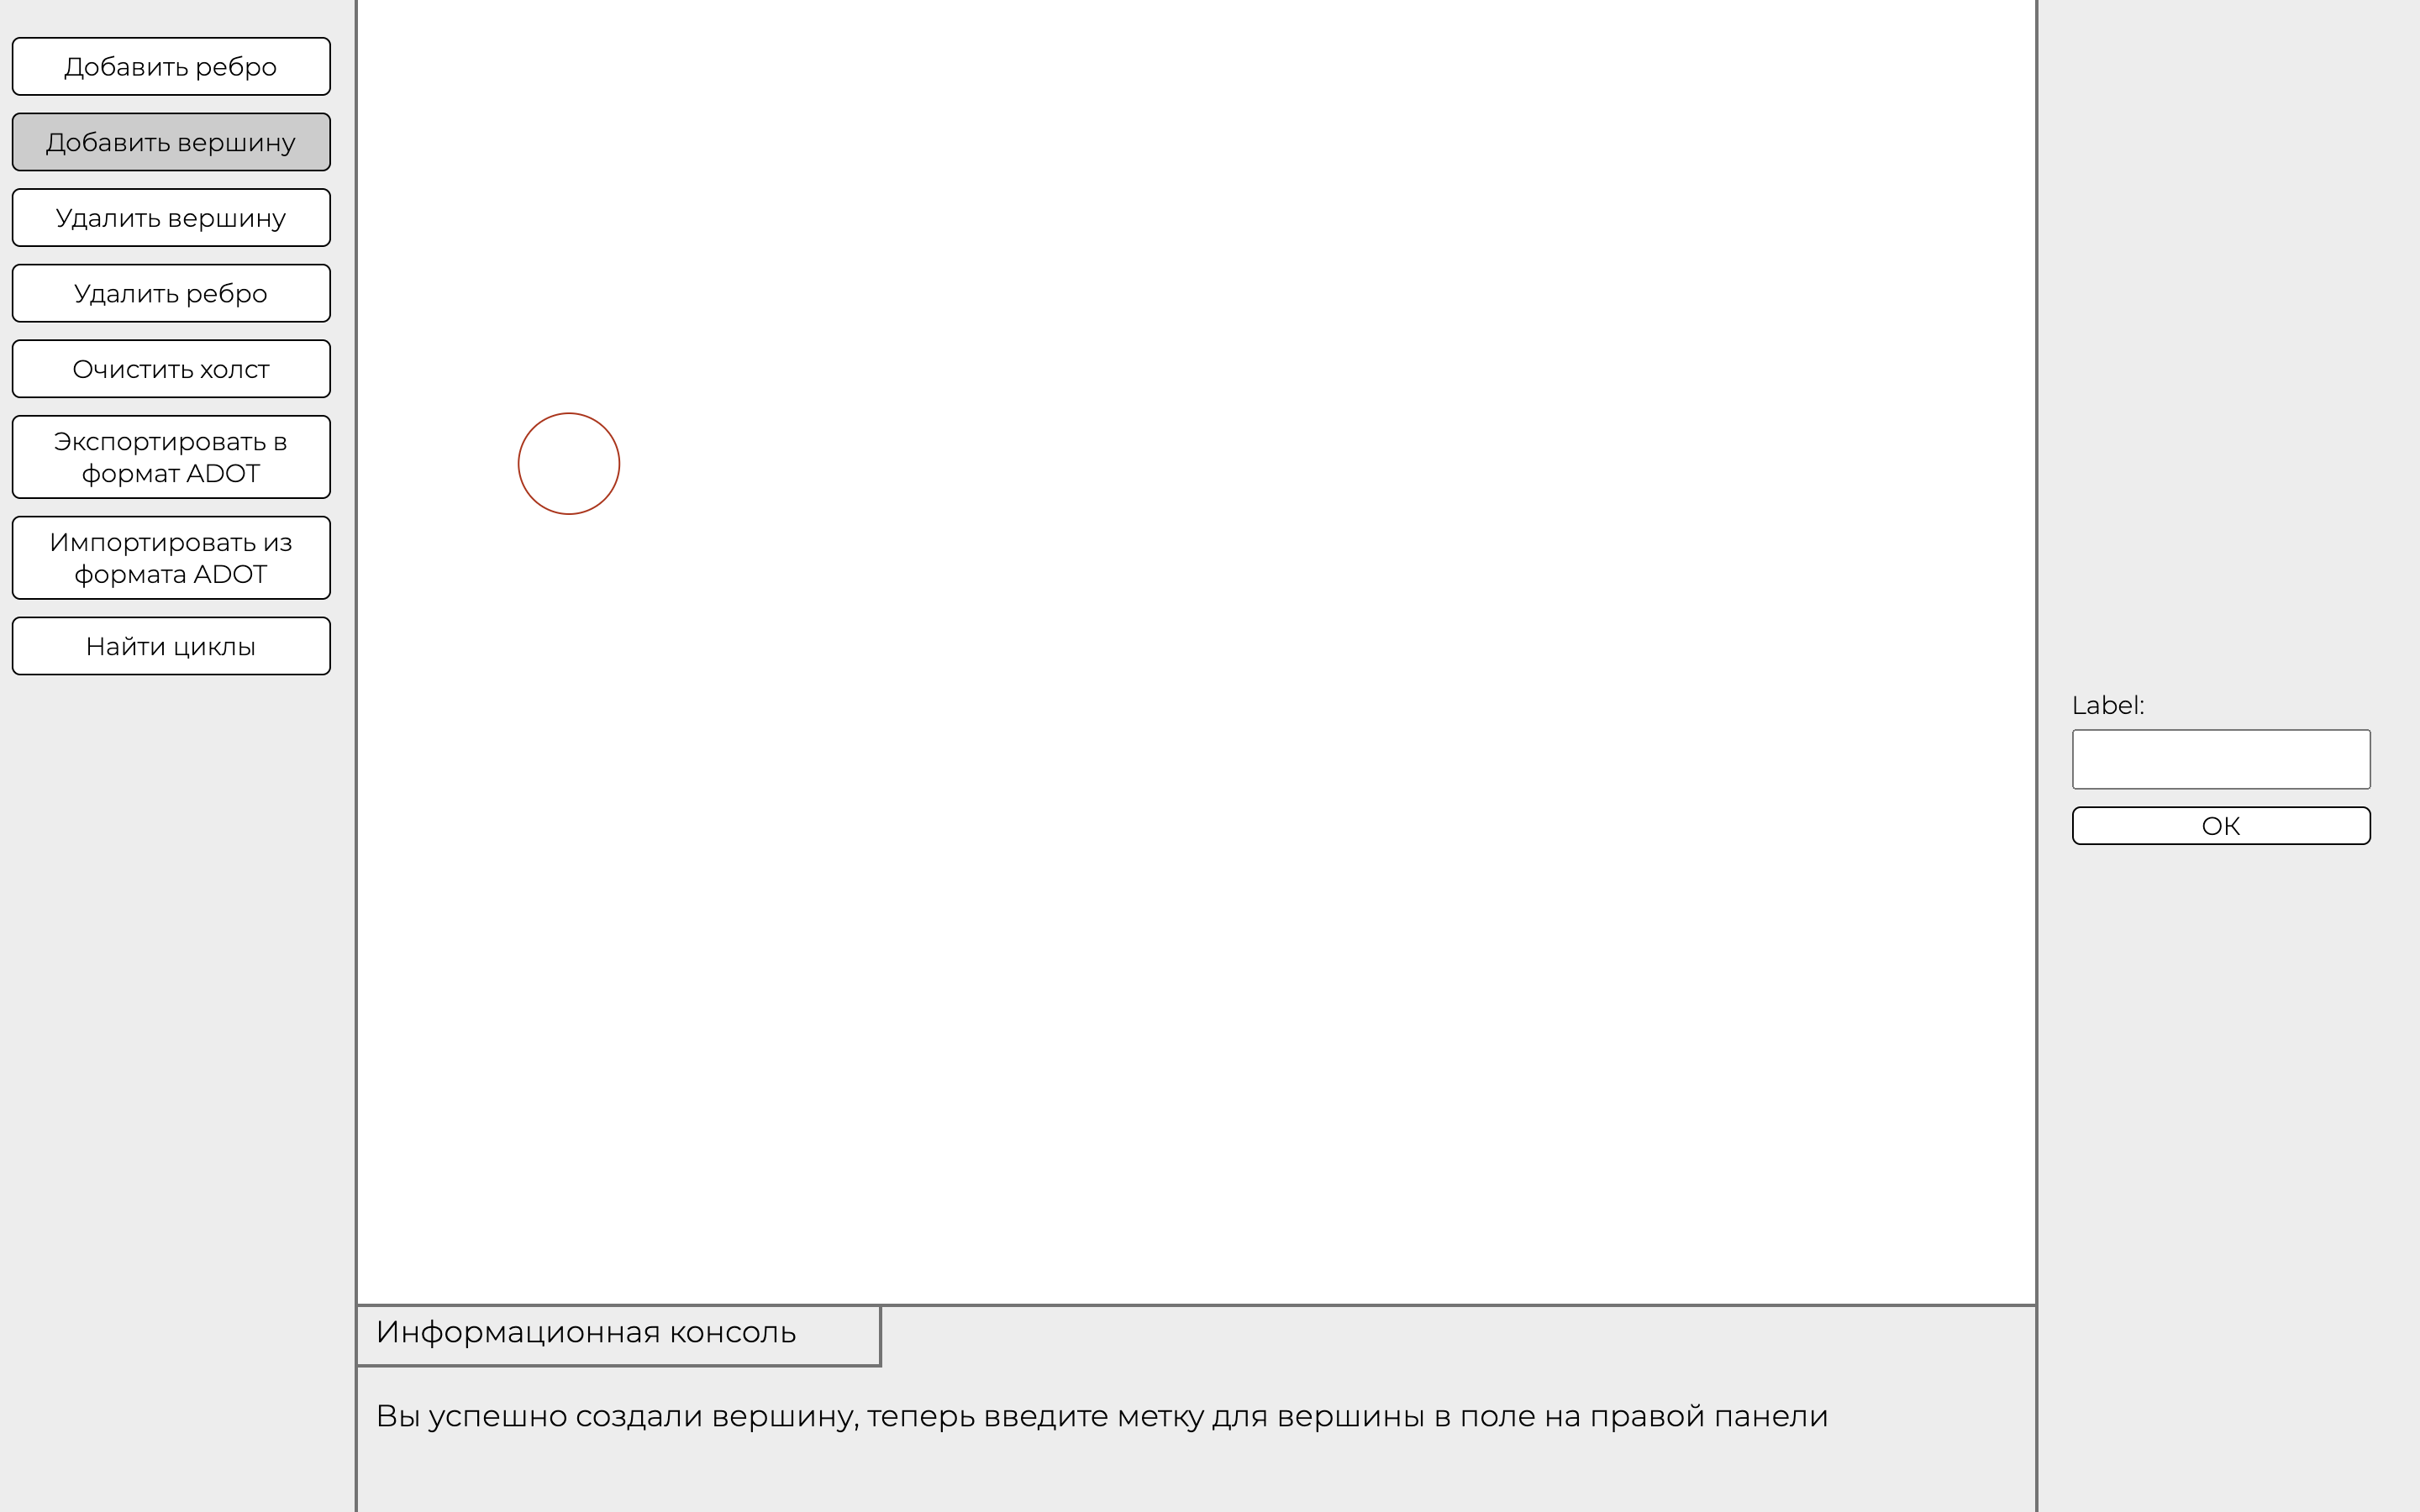
\includegraphics[width=0.9\linewidth]{ResearchNotes/images/vertex_create_1.png}}
\caption{Создание вершины}
\label{fig:vertex_create_1}
\end{figure}

Дополнительный функционал сценария:
\begin{itemize}
	\item Блокировка создания вершины если она находится в близости к другой вершине
	\item Блокировка создания названия вершины, если такое название присвоено существующей вершине
\end{itemize}

Сложности при реализации сценария:
\begin{itemize}
	\item Валидировать все необходимые параметры в процессе создания вершины: положение вершины, название вершины
	\item Выбор информации о вершине, которую нужно сохранить в оперативной памяти для дальнейшего использования в других сценариях
\end{itemize}

Будущее расширение функционала сценария:
\begin{itemize}
	\item Возможность изменить положение вершины в процессе ее создания. На данный момент вершина создается в месте клика на холст (в том случае если местоположение вершины валидно) и это местоположение уже никак нельзя изменить.
	\item Использование набора горячих клавиш для ускорения процесса создания вершины
	\item При  названия подсказать пользователю название вершины, в том случае если прошлые названия имеют инкрементирующийся для каждой вершины постфикс, например, уже созданы вершины $s_1, s_2$, при создании новой вершины в поле ввода названия система предложит пользователю название $s_3$.
\end{itemize}

\textbf{Добавление ребра}

Для добавления ребра необходимо поочередно выбрать две вершины, которые будут соединены ребром. Затем система потребует ввода предиката и функции, в том случае если введенный предикат или функция являются уникальнальными в рамках графа, то система потребует ввода информации о module и entry func. После этого построение ребра будет завершено. Процесс построения ребра представлен на рисунке \ref{fig:edge_create}.

\begin{figure}[h!]
\center{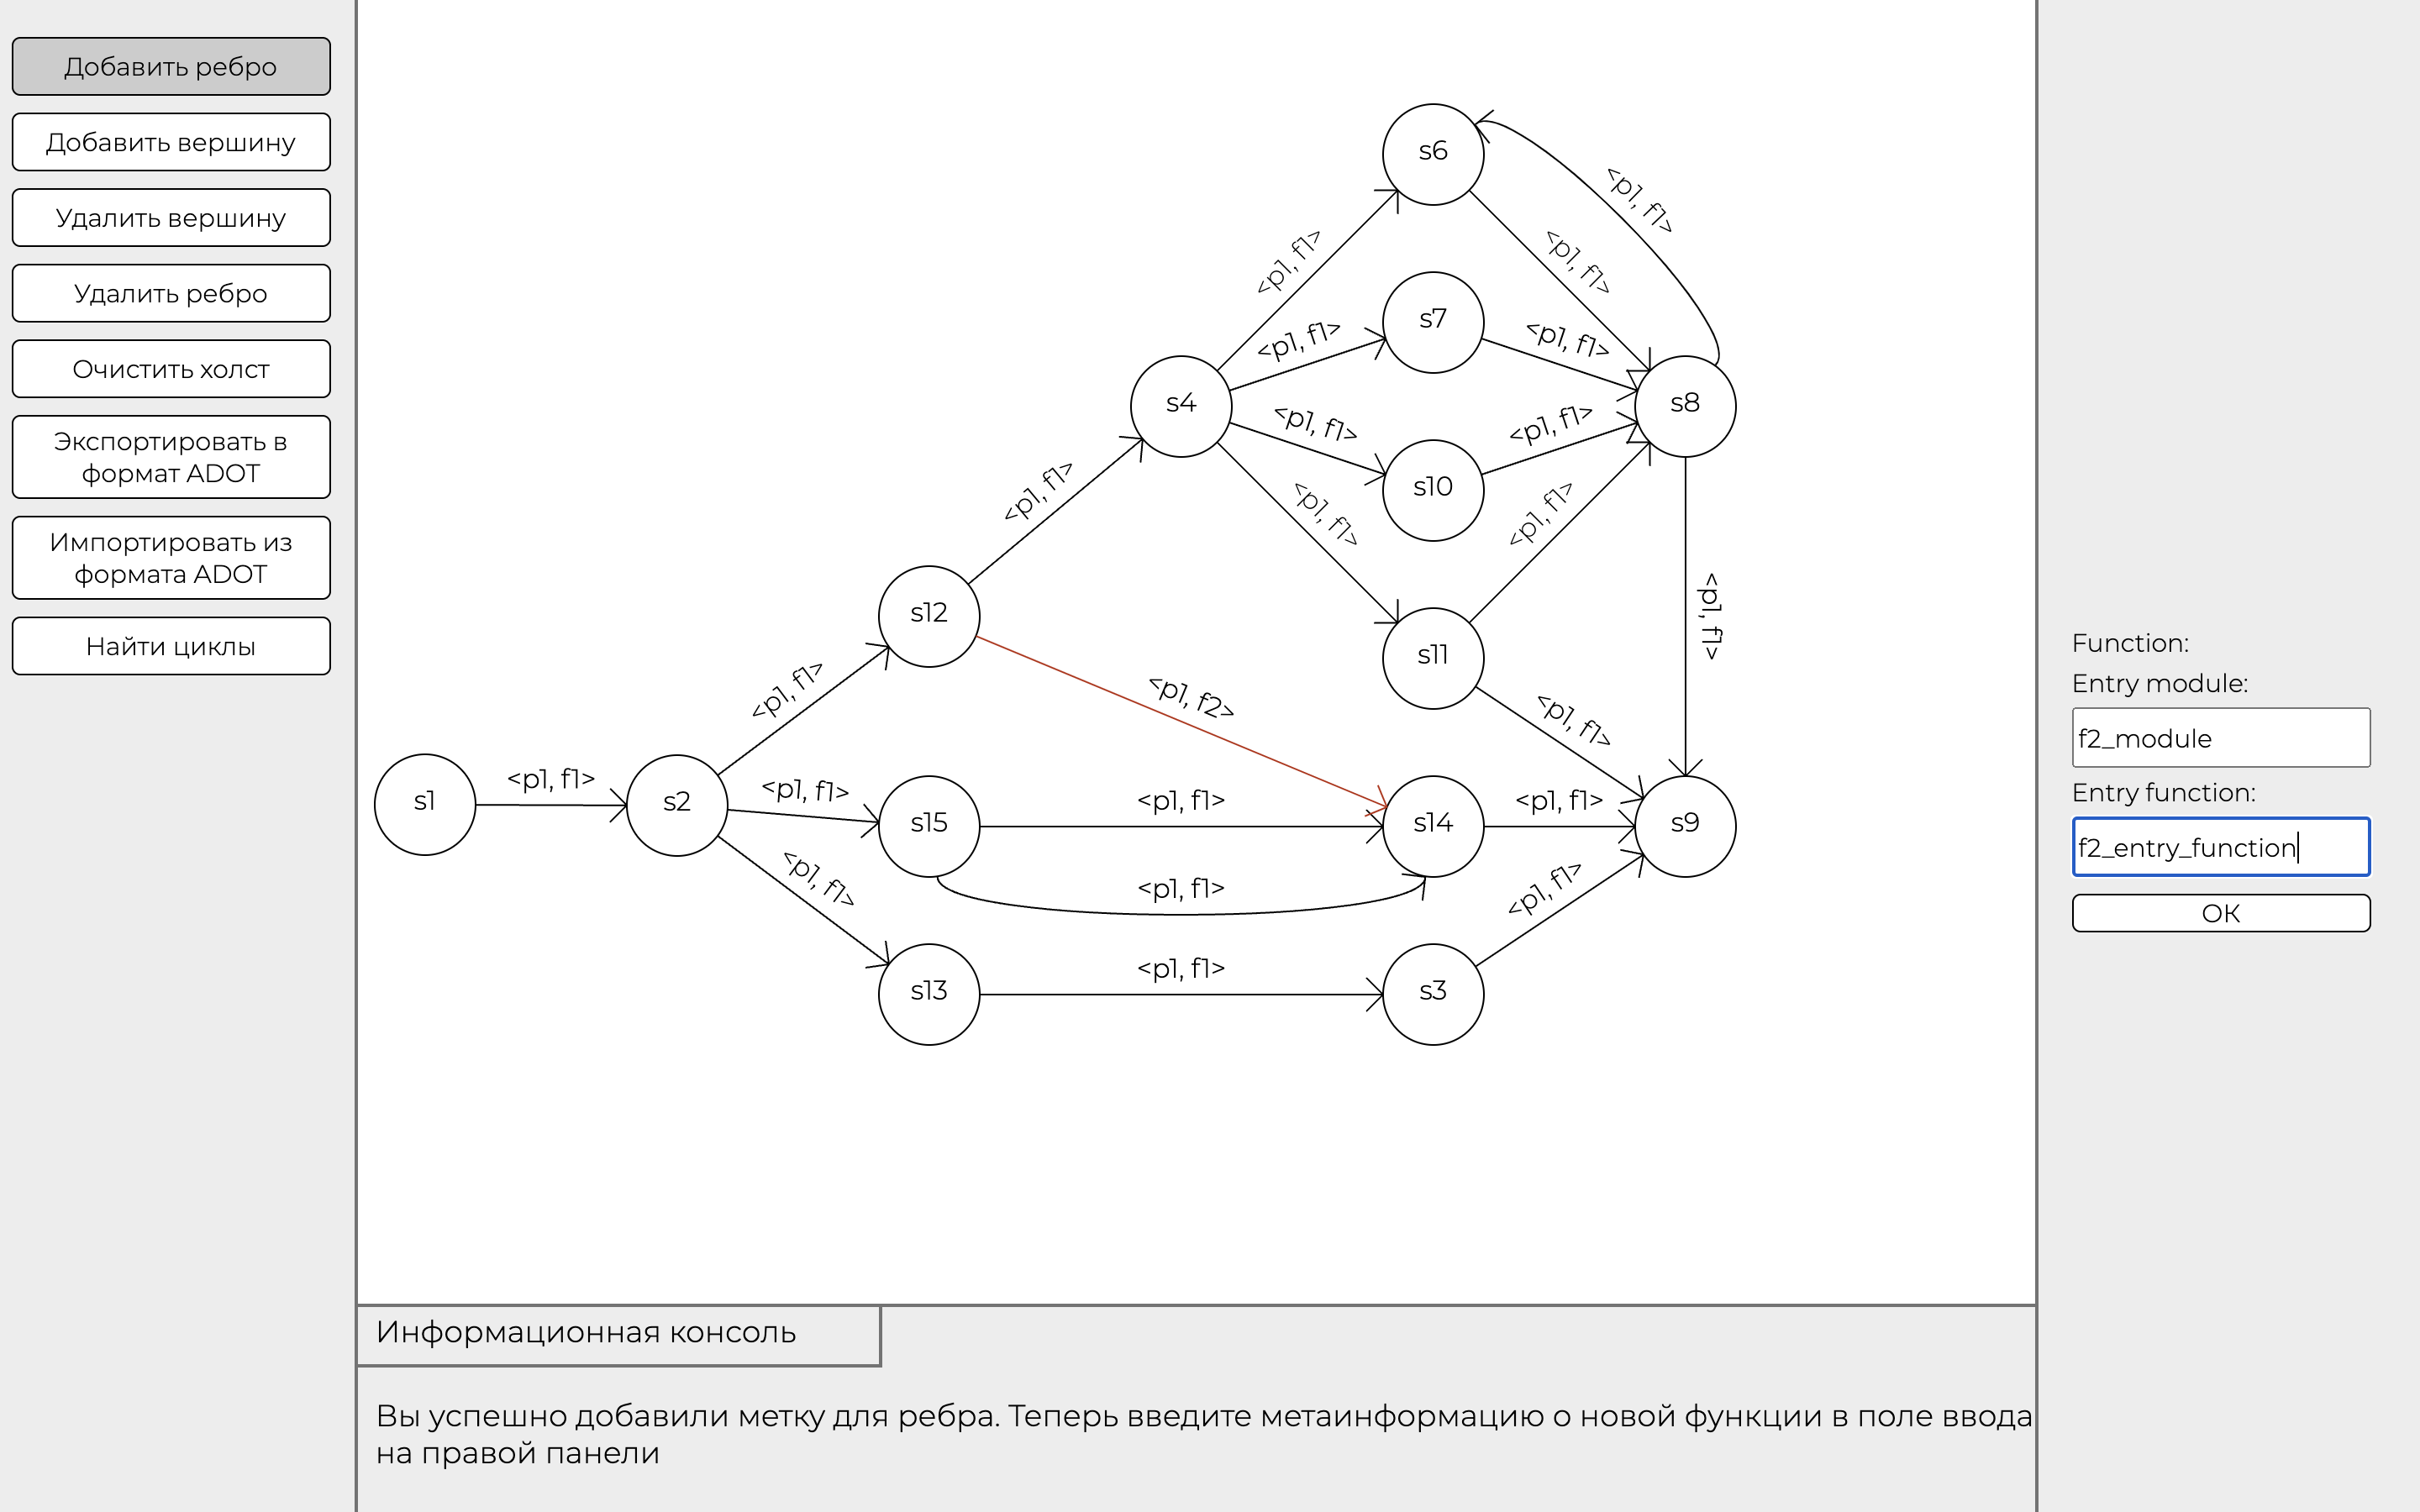
\includegraphics[width=0.9\linewidth]{ResearchNotes/images/edge_create.png}}
\caption{Создание ребра}
\label{fig:edge_create}
\end{figure}

Дополнительный функционал сценария:
\begin{itemize}
	\item Блокировка создания ребра из вершины в нее же саму.
	\item Если между вершинами уже существуют ребра, то система построит ребро, используя кривые Безье.
	\item Если на момент построения ребра из вершины выходит только одно ребро, то система потребует учтонения типа параллелизма (формат aDOT).
	\item Если предикат или функция не являются уникальными в рамках графа, то не требуется уточнение информации о module и entry func.
\end{itemize}

Сложности при реализации сценария:
\begin{itemize}
	\item Использование множества вспомогательных функций: подсчет количества ребер между вершинами, для определения типа построения ребра (прямое или кривые Безье), подсчет количества ребер выходящих из вершины для уточнения типа параллелизма, проверка полей ввода предиката и функции (предикат может быть неопределен, а функция должна быть определена), проверка введенных предиката и функции на уникальность в рамках графа.
	\item Выбор типа построения ребра: прямое, кривые Безье. Обработка ситуации, когда пользователь создает цикл между этими вершинами.
\end{itemize}

Будущее расширение функционала сценария:
\begin{itemize}
	\item Возможность перевыбора вершин для построения ребра между ними. На данный момент нельзя допустить ошибку при выборе вершин, необходимо закончить процесс построения ребра, удалить его и создать новое, выбрав другие вершины.
	\item Алгоритм для построения ребра с использованием кривых Безье. На данный момент ребро строится с помощью одной кривой Безье, что не позволяет строить ребра более сложного вида, тем самым разрешая коллизии, когда ребро проходит через другие вершины.
\end{itemize}

\textbf{Удаление вершины}

Для удаления вершины необходимо выбрать соответствующий пункт в меню, а затем кликнуть на вершину для удаления - вершина удаляется с холста вместе со всеми связанными с ней ребрами.

Сложности при реализации сценария:
\begin{itemize}
	\item Корректно удалить все связанные с вершиной ребра, а затем удалить информацию об этих ребрах и связанных вершин.
\end{itemize}

Будущее расширение функционала сценария:
\begin{itemize}
	\item Возможность одновременного выбора нескольких вершин для удаления.
	\item Возможность откатить действия в том случае если была удалена лишняя вершина. В целом это касается всего приложения, на данный момент любое действие неотвратимо.
\end{itemize}

\textbf{Удаление ребра}

Для удаления ребра необходимо выбрать соответствующий пункт в меню, а затем клкинуть на ребро для удаления - ребро удаляется с холста.

Сложности при реализации сценария:
\begin{itemize}
	\item Удалить информацию о ребре из связанных этим ребром вершин.
\end{itemize}

Будущее расширение функционала сценария:
\begin{itemize}
	\item Более корректный выбор ребра, на данный момент надо кликать ровно на ребро поскольку для перехвата события клика используется event.target.closest
	\item Возможность одновременного выбора нескольких ребер для удаления
\end{itemize}

\textbf{Экспорт в формат aDOT}

Для экспорта в формат aDOT необходимо выбрать соответствующий пункт в меню, а затем поочередно выбрать две вершины, которые будут являться стартовой и конечной вершиной соответственно. Затем сформируется текстовый файл с описание графа в формате aDOT и автоматически начнется его загрузка.

\textbf{Импорт из формата aDOT}

Для импорта из формата aDOT необходимо выбрать соответствующий пункт в меню, а затем выбрать файл для импорта. Далее система сама построит граф, сохранив всю необходимую информацию.

Сложности при реализации сценария:
\begin{itemize}
	\item Разработка алгоритма визуализации
\end{itemize}

Будущее расширение функционала сценария:
\begin{itemize}
	\item Разработка более гибкого алгоритма визуализации, который сможет работать с более сложными графами.
\end{itemize}


















%----------------------------------------------------------
\def\notedate{2022.04.25}
\def\currentauthor{Ершов В. (РК6-82Б)}
%----------------------------------------------------------
\notestatement{rndhpcedt}{Использование алгоритма DFS для решения задачи поиска циклов в ориентированном графе}

Для поиска циклов в ориентированном графе необходим алгоритм обхода графа. Обход графа - это переход от одной вершины графа к другой с целью поиска ребер или вершин, которые удовлетворяют некоторому условию.

Основными алгоритмами обхода графа являются поиск в ширину (Breadth-First Search, BFS) и поиск в глубину (Depth-First Search). Основное различие между DFS и BFS состоит в том, что DFS проходит путь от начальной вершины до конечной, а BFS двигается вперед уровень за уровнем. Из этого следует, что алгоритмы применяются для решения разных задач. BFS используется для более эффективного нахождения кратчайшего пути в графе, определения связанных компонент в графе, а также обнаружения двудольного графа. DFS применяется для проверки графа на ацикличность или для решения задачи поиска циклов в графе.

Как ранее было сказано, алгоритм DFS двигается от начальной вершины до тех пор пока не будет достигнута конечная вершина. Если был достигнут конец пути, но искомая вершина так и не была найдена, то необходимо вернуться назад (к точке разветвления) и пойти по другому маршруту. Рассмотрим работу алгоритма на примере:

\begin{figure}[H]
\center{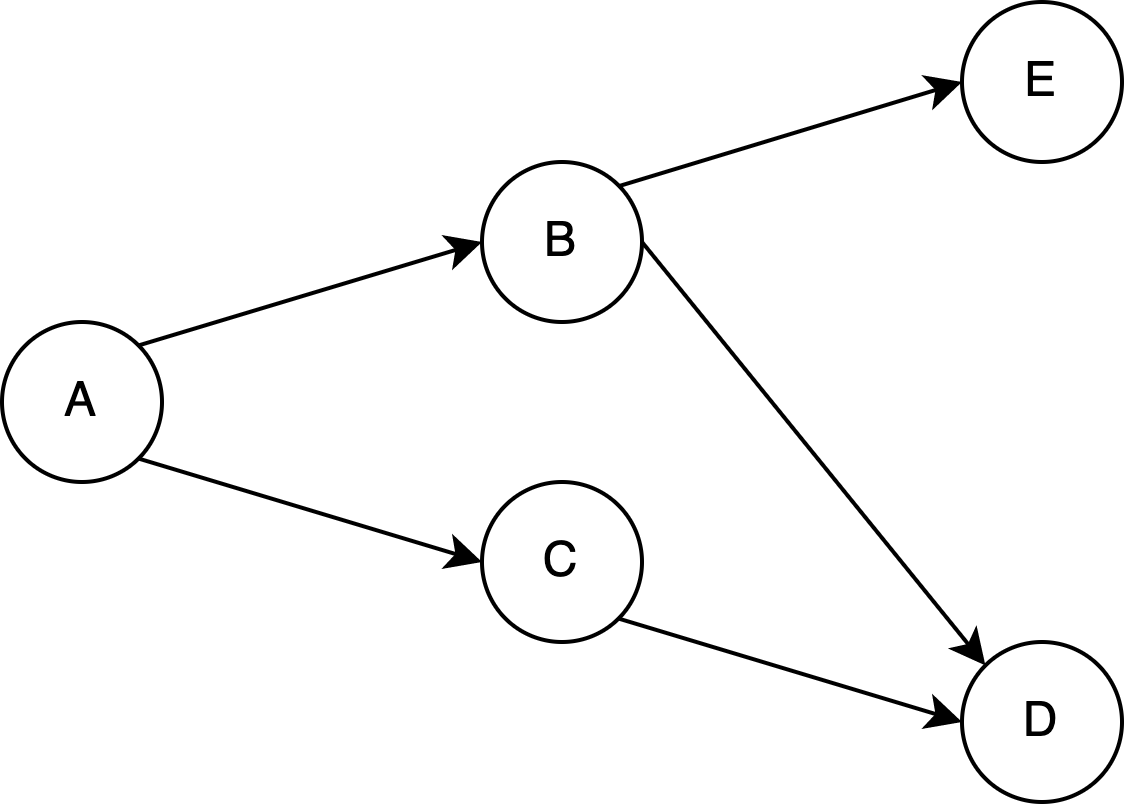
\includegraphics[width=0.7\linewidth]{ResearchNotes/rndhpc_not_edt_2022_04_25/dfs_1.png}}
\end{figure}

Мы находимся в точке ``A'' и хотим найти вершину ``E''. Согласно принципу DFS, необходимо исследовать один из возможных маршрутов до конца, если не будет обнаружена вершина ``E'', то возвращаемся и исследуем другой маршрут.

\begin{figure}[H]
\center{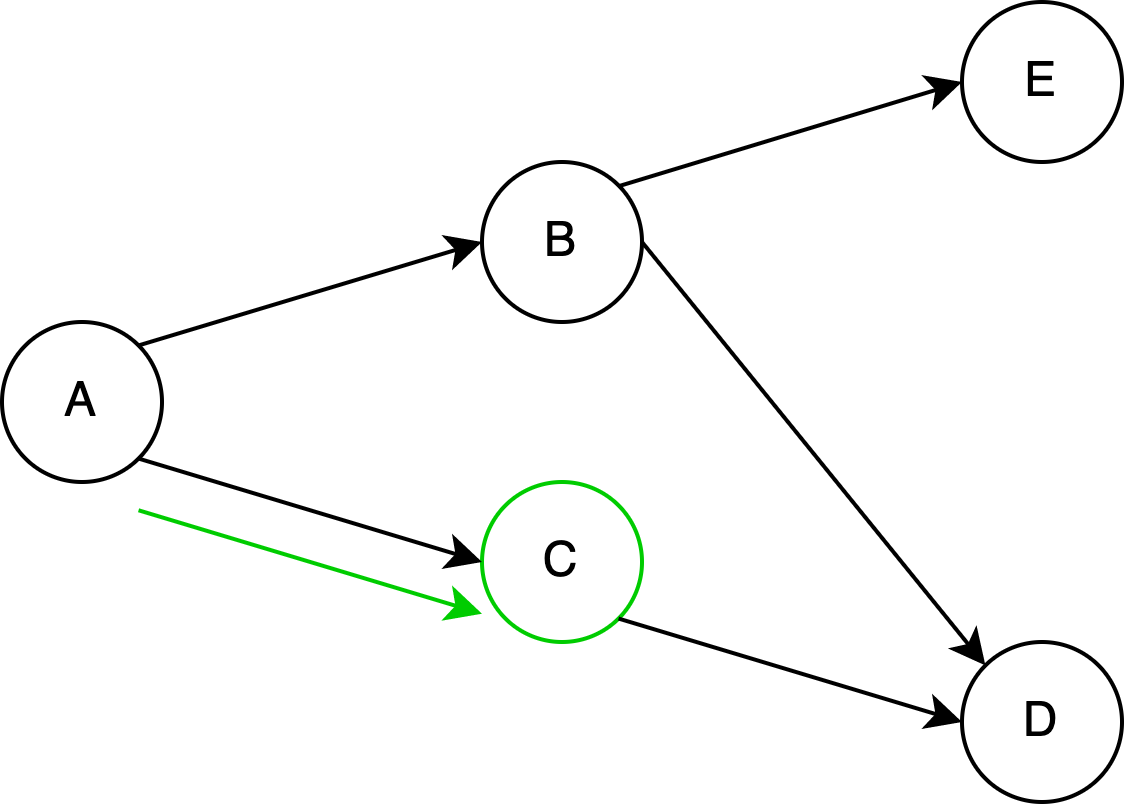
\includegraphics[width=0.7\linewidth]{ResearchNotes/rndhpc_not_edt_2022_04_25/dfs_2.png}}
\end{figure}

В данном случае мы двигаемся к ближайшей вершине ``C'', поскольку это не конец пути, то переходим к следующей вершине.

\begin{figure}[H]
\center{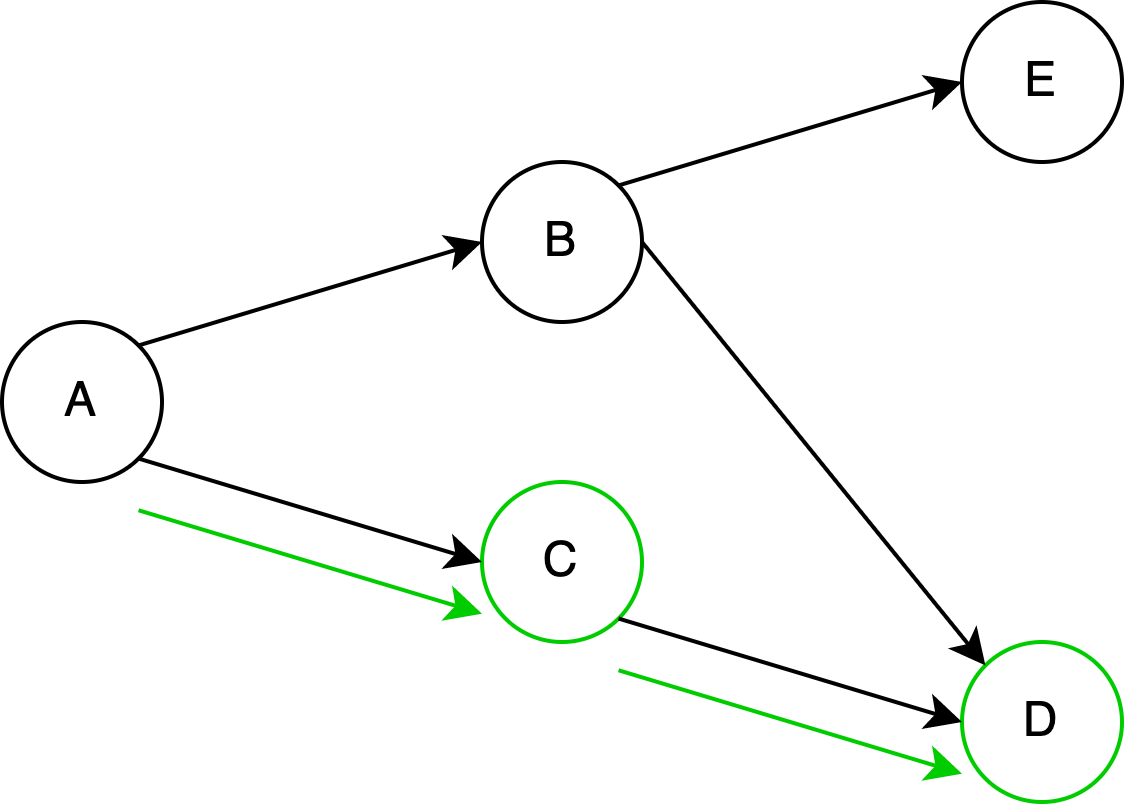
\includegraphics[width=0.7\linewidth]{ResearchNotes/rndhpc_not_edt_2022_04_25/dfs_3.png}}
\end{figure}

Мы достигли конца пути, но не нашли ``E'', поэтому возвращаемся в начальную вершину ``A'' и двигаемся по другому пути.

\begin{figure}[H]
\center{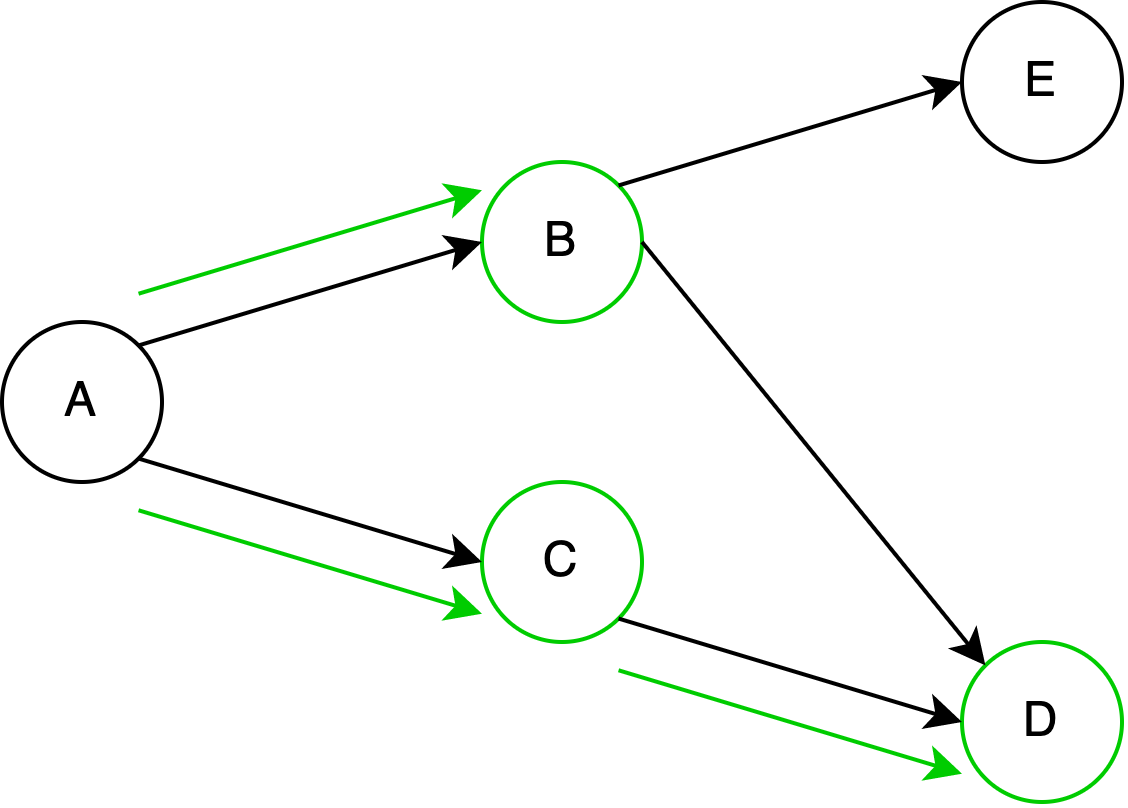
\includegraphics[width=0.7\linewidth]{ResearchNotes/rndhpc_not_edt_2022_04_25/dfs_4.png}}
\end{figure}

Из вершины ``B'' существует два возможных дальнейших пути. Поскольку вершина ``D'' была ранее расмотрена двигаемся по другому пути.

\begin{figure}[H]
\center{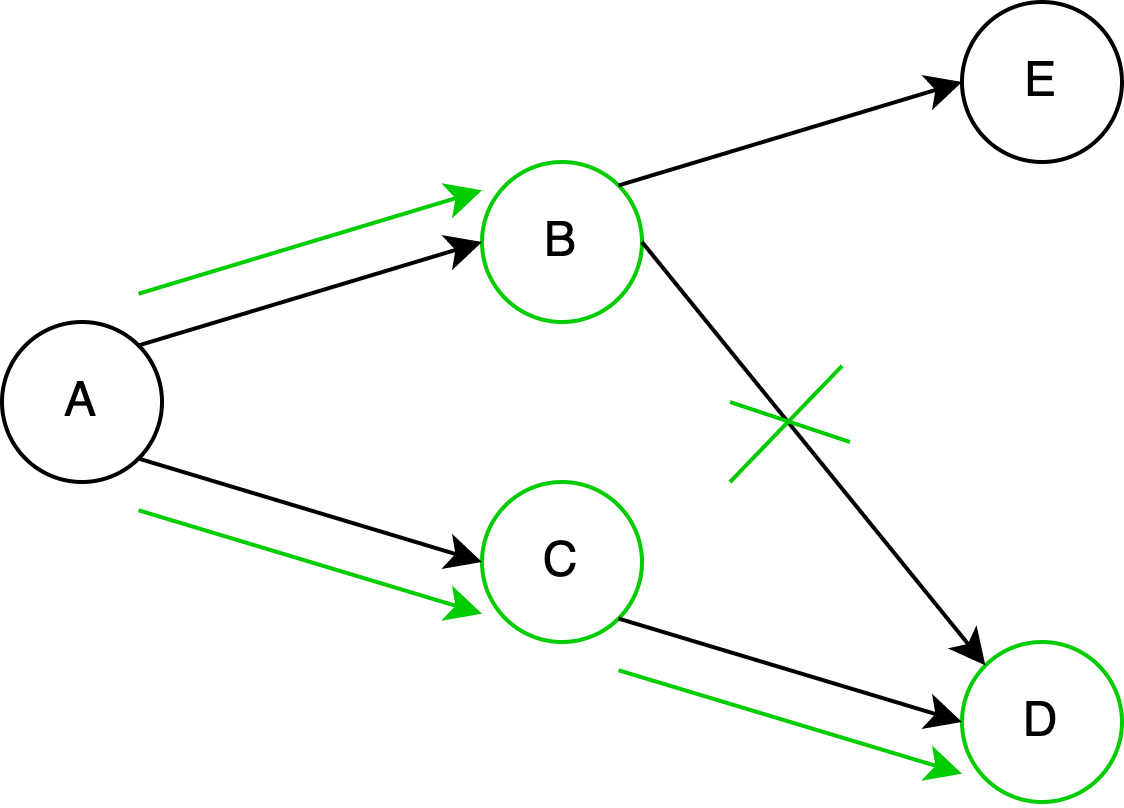
\includegraphics[width=0.7\linewidth]{ResearchNotes/rndhpc_not_edt_2022_04_25/dfs_5.png}}
\end{figure}

\begin{figure}[H]
\center{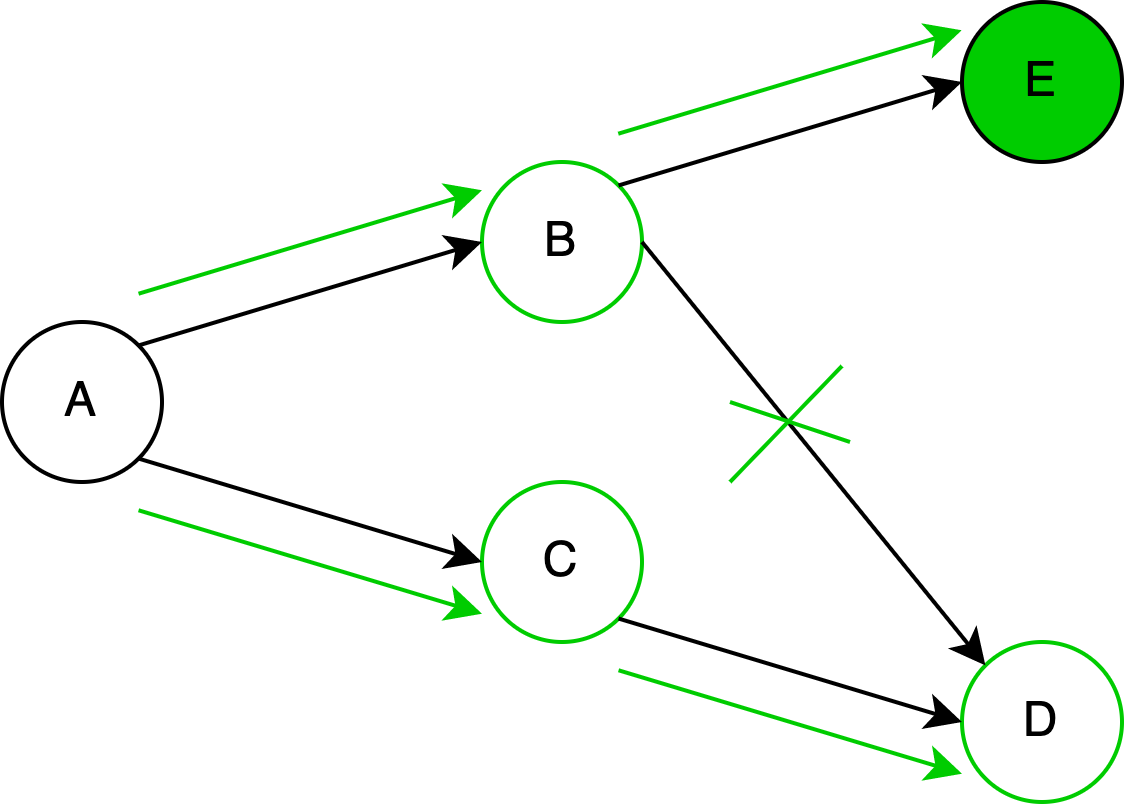
\includegraphics[width=0.7\linewidth]{ResearchNotes/rndhpc_not_edt_2022_04_25/dfs_6.png}}
\end{figure}

Мы нашли искомую вершину ``E'', следовательно можно завершать выполнение алгоритма.

В рассмотреном примере решалась достаточно тривиальная задача - поиск вершины в графе.
Более интересной является задача поиска циклов в графе. Каждая вершина графа может находиться в трех различных состояниях: вершина не посещена, вершина посещена и вершина посещена, но мы не дошли до конца пути, который включает эту вершину. Для ясности введем следующие обозначения состояний:
\begin{itemize}
	\item NOT_VISITED - вершина еще не посещена;
	\item IN_STACK - вершина посещена, но мы не дошли до конца пути;
	\item VISITED - вершина посещена.
\end{itemize}

Если в процессе обхода мы встречаем вершину, которая помечена как ``IN_STACK'', то мы нашли цикл.

В программной реализации рационально разбить задачу на три функции:
\begin{itemize}
	\item Функция, которая в цикле проходит по всем вершинам графа и если вершина не была ранее просмотрена, то запускает обход DFS из этой вершины
	\item Функция непосредственно реализующая обход DFS
	\item Функция для печати найденного цикла
\end{itemize}

Ниже приведен (листинг~\ref{lst:gm.exmpl.3}) кода данных функций на языке C++

\begin{lstlisting}[frame=single, label={lst:gm.exmpl.3}, caption={Решение задачи поиска циклов в ориентированном графе \textsf{G}}, language=C++]
void FindCycles(const std::vector<int> &adjacency_list)
{
    std::vector<std::string> visited(adjacency_list.size(), "NOT_VISITED");

    for (int vertex = 0; vertex < adjacency_list.size(); ++vertex)
    {
        if (visited[vertex] == "NOT_VISITED")
        {
            std::stack<int> stack;
            stack.push(vertex);
            visited[vertex] = "IN_STACK";
            processDFS(adjacency_list, visited, stack);
        }
    }
}

void processDFS(const std::vector<int> &adjacency_list,
                std::vector<std::string> &visited,
                std::stack<int> &stack)
{
    for (const int &vertex : adjacency_list[stack.top()])
    {
        if (visited[vertex] == "IN_STACK")
        {
            printCycle(stack, vertex);
        }
        else if (visited[vertex] == "NOT_VISITED")
        {
            stack.push(vertex);
            visited[vertex] = "IN_STACK";
            processDFS(adjacency_list, visited, stack);
        }
    }

    visited[stack.top()] = "DONE";
    stack.pop();
}

void printCycle(std::stack<int>& stack, int vertex)
{
    std::stack<int> stack_temp;
    stack_temp.push(stack.top());
    stack.pop();

    while (stack_temp.top() != vertex)
    {
        stack_temp.push(stack.top());
        stack.pop();
    }

    while (!stack_temp.empty())
    {
        std::cout << stack_temp.top() << ' ';
        stack.push(stack_temp.top());
        stack_temp.pop();
    }

    std::cout << '\n';
}
\end{lstlisting}

%-------------------------------------

%----------------------------------------------------------
% Атрибуты задачи
\noteattributes{}
%----------------------------------------------------------

%----------------------------------------------------------
\section{\rndprojectdscr{rndhpcpar}}

%----------------------------------------------------------
\def\notedate{2021.11.14}
\def\currentauthor{Муха В. (РК6-73Б)}
%----------------------------------------------------------
\notestatement{rndhpcedt}{Известные алгоритмы поиска циклов в ориентированных графах}
%----------------------------------------------------------
%\subsubsection{}

Существует несколько групп алгоритмов поиска\cite{davidrajuh2016}:
\begin{enumerate}[label=\arabic*)]
    \item алгоритмы, основанные на обходе ориентированного графа (ОГ);
    \item алгоритмы, основанные на использовании матриц смежности, описывающих конкретный граф.
\end{enumerate}

Одним из представителей алгоритмов первой группы (обхода ОГ) является алгоритм поиска в глубину (англ., depth-first-search (DFS)), который предполагает, что обход осуществляется из фиксированного и заранее заданного узла. Если число узлов ОГ равно $n$, то сложность алгоритма DFS $O(n^2)$ и $O(n^3)$ -- для случая ``многократного обхода'' из каждого узла\footnote{Для случая ОГ возможность идентификации всех циклов требует осуществления многократных обходов, начиная с каждого из узлов ОГ.}. Поэтому для ускорения алгоритма необходимо применение модификаций, например распараллеливание алгоритма поиска в глубину~\cite{Mahdi2011}.

%Предполагая далее, что $n$ число узлов, з
Зададим граф $G(V, E)$, где $V = \{\bs{a}, \bs{b}, \bs{c}, \ldots\}$ -- множество вершин, $|V|=n$, а $E = \{\alpha\beta: \alpha\beta\in V\times V\}$ -- множество рёбер (пример, $\{\bs{ab}, \bs{ad}, \ldots , \bs{ge}\}$).

Для определения ОГ, часто, применяют понятие матриц смежности\cite{diestel2012graph}:
\begin{equation}\label{eq.rndhpcpar.2021.11.14.01}
\begin{array}{l}
||A||=||a_{ij}||_{n\times n};\\
a_{ij}=\left\{\begin{array}{l} 1, \mbox{ -- определено ребро с началом в узле $i$ и концом в узле $j$};\\ 0, \mbox{ -- ребро не определено}.\end{array} \right.
\end{array}
\end{equation}

\begin{equation}\label{eq.rndhpcedt.2021.11.14.00}
A=%
\begin{bmatrix}
	&	\bs{a}	&	\bs{b}	&	\bs{c}	&	\bs{d}	&	\bs{e}	&	\bs{f}	&	\bs{g} \\
\bs{a}	&	0	&	1	&	0	& 	1	& 	0	& 	0	 &	 0 \\
\bs{b}	&	0	&	0	&	0	& 	0	& 	1	& 	0	 &	 1 \\
\bs{c}	&	0	&	0	&	0	& 	0	& 	0	& 	1	 &	 0 \\
\bs{d}	&	1	&	0	&	1	& 	0	& 	0	& 	0	 &	 0 \\
\bs{e}	&	0	&	0	&	0	& 	0	& 	0	& 	1	 &	 0 \\
\bs{f}	&	0	&	0	&	1	& 	0	& 	0	& 	0	 &	 0 \\
\bs{g}	&	0	&	0	&	1	& 	1	& 	1	& 	01	 &	 0 \\
\end{bmatrix}
\end{equation}

Пример графа, построенного на основе его матрицы смежности $A$, приведен на рис.~\ref{fig.rndhpcpar.2021.11.14.01}.

%\begin{figure}[!ht]
%	\centering
%	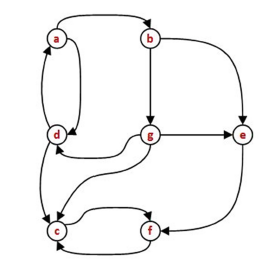
\includegraphics[width=0.3\textwidth]{ResearchNotes/rndhpc_not_par_2021_11_14/adj_matrix.png}
%	\caption{Граф, построенный по матрице смежности A}\label{fig.rndhpcpar.2021.11.14.01}
%\end{figure}

\begin{figure}[!ht]
	\centering
	\tikzstyle{circ} = [circle, text centered, draw=black]
	\tikzstyle{ar} = [->, >={Stealth[length=7pt]}]
	\tikzstyle{nt} = [text centered, color=black!50]
	\begin{tikzpicture}[align=center, auto]%, scale=1.16]
		\node[circ] (a) at (0,0) {$a$};
		\node[circ] (b) at (2,0) {$b$};
		\node[circ] (d) at (0,-2) {$d$};
		\node[circ] (g) at (2,-2) {$g$};
		\node[circ] (e) at (4,-2) {$e$};
		\node[circ] (c) at (0,-4) {$c$};
		\node[circ] (f) at (2,-4) {$f$};
		\draw [ar] (a) edge [bend left] (b);
		\draw [ar] (a) edge [bend left] (d);
		\draw [ar] (d) edge [bend left] (a);
		\draw [ar] (g) edge [bend left] (d);
		\draw [ar] (b) edge (g);
		\draw [ar] (g) edge (e);
		\draw [ar] (e) edge [bend left] (f);
		\draw [ar] (c) edge [bend left] (f);
		\draw [ar] (f) edge [bend left] (c);
		\draw [ar] (g) edge (c);
		\draw [ar] (d) edge [bend right] (c);
	\end{tikzpicture}
	\caption{Граф, построенный по матрице смежности A}\label{fig.rndhpcpar.2021.11.14.01}
\end{figure}

Элемент матрицы смежности $a_{ij}$ указывает на факт наличия определённого рёбра с началом в узле $i$ и концом в узле $j$, тогда как транспонированная матрица $A^T$ задаёт новый ОГ с теми же узлами и рёбрами, противоположно направленными относительно исходного ОГ.

\begin{equation}\label{eq.rndhpcpar.2021.11.14.02}
	A^T=%
	\begin{bmatrix}
		&	\bs{a}	&	\bs{b}	&	\bs{c}	&	\bs{d}	&	\bs{e}	&	\bs{f}	&	\bs{g} \\
	\bs{a}	&	0	&	0	&	0	& 	1	& 	0	& 	0	 & 	0 \\
	\bs{b}	&	1	&	0	&	0	& 	0	& 	0	& 	0	 & 	0 \\
	\bs{c}	&	0	&	0	&	0	& 	1	& 	0	& 	1	 & 	1 \\
	\bs{d}	&	1	&	0	&	0	& 	0	& 	0	& 	0	 & 	1 \\
	\bs{e}	&	0	&	1	&	0	& 	0	& 	0	& 	0	 & 	1 \\
	\bs{f}	&	0	&	0	&	1	& 	0	& 	1	& 	0	 & 	0 \\
	\bs{g}	&	0	&	1	&	0	& 	0	& 	0	& 	0	 & 	0 \\
	\end{bmatrix}
	\end{equation}

Введём обозначение матрицы, возведённой в степень $m$:
\begin{equation}\label{eq.rndhpcpar.2021.11.14.03}
A^m=\underbrace{A\times A \times \ldots \times A}_{m}.
\end{equation}

Матрица $A^m$ обладает следующим свойством: элемент матрицы $a^i_j$ равен числу путей из вершины $i$ в вершину $j$, состоящих ровно из $m$ рёбер\cite{diestel2012graph}. Длиной цикла называют количстево рёбер в этом цикле. Для того, чтобы определить циклы длины $2m$, нужно найти матрицу циклов $C_m$, определяемую следующим образом: 

\begin{equation}\label{eq.rndhpcpar.2021.11.14.04}
    C_m = A^m \wedge (A^T)^m;
\end{equation}
где $\wedge$ -- оператор конъюнкции, применяемый поэлементно.

Таким образом, матрица $C_m$ будет содержать все циклы длины $2m$. Пример для поиска циклов длины 2.~\ref{eq.rndhpcpar.2021.11.14.05}.
\begin{equation}\label{eq.rndhpcpar.2021.11.14.05}
	C_2 = A \wedge A^T = %
	\begin{bmatrix}
		&	\bs{a}	&	\bs{b}	&	\bs{c}	&	\bs{d}	&	\bs{e}	&	\bs{f}	&	\bs{g} \\
	\bs{a}	&	0	&	0	&	0	& 	1	& 	0	& 	0	 & 	0 \\
	\bs{b}	&	0	&	0	&	0	& 	0	& 	0	& 	0	 & 	0 \\
	\bs{c}	&	0	&	0	&	0	& 	0	& 	0	& 	1	 & 	0 \\
	\bs{d}	&	1	&	0	&	0	& 	0	& 	0	& 	0	 & 	0 \\
	\bs{e}	&	0	&	0	&	0	& 	0	& 	0	& 	0	 & 	0 \\
	\bs{f}	&	0	&	0	&	1	& 	0	& 	0	& 	0	 & 	0 \\
	\bs{g}	&	0	&	0	&	0	& 	0	& 	0	& 	0	 & 	0 \\
	\end{bmatrix}
	\end{equation}

%----------------------------------------------------------
% Атрибуты задачи
\noteattributes{}
%----------------------------------------------------------

%\input{ResearchNotes/rndhpc_not_edt_@year@_@month@_@id@.tex}

%----------------------------------------------------------
\section{\rndprojectdscr{rndhpcblo}}

%----------------------------------------------------------
\def\notedate{2021.11.06}
\def\currentauthor{Тришин И.В. (РК6)}%
%----------------------------------------------------------
\notestatement{rndhpcblo}{Графовое описание процессов обработки данных в pSeven (DATADVANCE)} 

\textsf{pSeven} -- это платформа для анализа данных, оптимизации и создания аппроксимационных моделей, дополняющая средства проектирования и инженерного анализа.
\textsf{pSeven} позволяет интегрировать в единой программной среде различные инженерные приложения, алгоритмы многодисциплинарной оптимизации и инструменты анализа данных для упрощения принятия конструкторских решений~\cite{DatadvanceOffWebsite2021}.

%--------------------------------
\subsubsection{Принципы функционирования}

На концептуальном уровне в \textsf{pSeven} вводятся следующие понятия.
\begin{itemize}
    \item Проект -- набор файлов, используемых в \textsf{pSeven} для описания решений одной или нескольких задач и хранения результатов их решения.
    \item Расчётная схема (workflow) -- формальное описание процесса решения некоторой задачи в виде ориентированного графа, узлами которого являются блоки, а рёбрами - связи. Такое описание хранится в бинарном файле с расширением \textsf{.p7wf}, использующем некоторый специализированный формат хранения подобного рода описаний.
    \item Блок -- функциональный элемент расчётной схемы, отвечающий за обработку входных данных и формирование выходных данных~\cite{pSevenDocsWorkflow2021}.
    \item Порт -- переменная определённого типа, описанная в блоке и имеющая в нём уникальное имя, значение которой может быть передано в другие блоки или получено от них через связи.
    \item Связь (link) -- одностороннее соединение между двумя портами, обеспечивающее передачу данных от одного к другому.
\end{itemize}

Проекты в \textsf{pSeven} имеют единую базу данных, куда записываются все результаты запусков расчётных схем и откуда берутся данные для их последующей презентации пользователю и их анализа. Для определения переменных, значения которых должны быть записаны в неё записаны, предусмотрены специализированные порты для самих расчётных схем, с которыми связываются те блоки, результаты выполнения которых интересуют пользователя.

Связи служат для маршрутизации данных. С их помощью осуществляется и взаимодействие между блоками и, кроме того, определяется очерёдность их запуска. В момент добавления связи в пакете \textsf{pSeven} выполняется проверка портов на совместимость. Они считаются совместимыми, если тип данных источника можно преобразовать к типу данных адресата~\cite{pSevenDocsWorkflow2021}.

%--------------------------------
\subsubsection{Поддержка циклов и ветвлений}

Расчётная схема может включать расчётные циклы. Для их создания применяются специализированные блоки, имеющие функциональную возможность управления запуском других блоков в теле цикла и принятия решения о его прекращении. Такие блоки называются управляющими блоками циклов. Одним из характерных примеров является \textit{оптимизационный цикл}, управление которым осуществляется из блока \textsf{Optimizer}~\cite{pSevenDocsWorkflow2021}, позволяющего, например, настроить максимальное число итераций или требуемую точность, как условия окончания.

Если речь идёт о задачах анализа данных, существует отдельный блок, обозначающий входную точку цикла (\textsf{Loop}). Такой цикл принимает на вход список наборов аргументов, каждый из которых будет обработан на соответствующем шаге цикла, и выдаёт список наборов выходных значений, которые сохраняются в базе данных проекта.

Кроме того, существует возможность включения в расчётную схему условного и безусловного ветвления. Первое достигается за счёт создания связей для подключения одного и того же порта вывода к различным портам ввода. В этом случае по каждой связи передаётся копия выходных данных, полученных у источника~\cite{pSevenDocsWorkflow2021}. Условные ветвления создаются с помощью специального блока \textsf{Condition}, который по определённому условию передаёт входные данные одному из подключенных блоков. Их целесообразно использовать для устранения ошибок в работе блока, отбраковки некорректных входных данных и других аналогичных целей~\cite{pSevenDocsWorkflow2021}.

%--------------------------------
\subsubsection{Особенности выполнения расчётных схем}

При выполнении расчётных схем каждый блок запускается в отдельном процессе на уровне операционной системы. Как сказано ранее, начало выполнения блока определяется его связями с другими. Любой блок будет ожидать завершения работы другого блока только в том случае, если ему необходимо получить от него входные данные. Это означает, что два блока, не имеющих связей друг с другом, входящие в состав различных ветвлений расчётной схемы, могут запускаться параллельно, поскольку они не зависят друг от друга по используемым данным~\cite{pSevenDocsWorkflow2021}.

Кроме того, при обработке больших выборок данных может потребоваться обрабатывать по несколько наборов данных одновременно в независимых потоках исполнения. Помимо прочего этой цели служит блок \textsf{Composite}, который является контейнером для нескольких блоков. В его настройках можно включить опцию параллельного исполнения, указать, с какого порта данные будут обрабатываться параллельно, и указать максимальное число потоков. При запуске расчётной схемы пакет \textsf{pSeven} создаёт несколько виртуальных экземпляров блока \textsf{Composite} и автоматически распределяет входные наборы данных между ними. Как только в одном из таких виртуальных блоков завершается расчёт, он получает из выборки следующий набор для обработки~\cite{pSevenDocsParallel2021}.

%----------------------------------------------------------
% Атрибуты задачи
\noteattributes{}
%----------------------------------------------------------

\def\notedate{2022.02.09}
\def\currentauthor{Тришин И.В. (РК6)}%
%----------------------------------------------------------
\notestatement{rndhpcblo}{Сравнительная характеристика GBSE, pSeven, Pradis}

В рамках сравнения были рассмотрены известные программные комплексы, в основе которых в том или ином виде лежит идея организации вычислений, описываемая с помощью ориентированных графов (графоориентированный подход).

Для проведения сравнения с GBSE~\cite{SokPersh2018GBSE} были выбраны следующие известные программные комплексы:\pdfcomment{Стоило бы указать подробнее причины такого выбора...}
\begin{enumerate}
    \item \textsf{Pradis} -- разработка отечественной компании ``Ладуга'';
    \item \textsf{pSeven} -- разработка отечественной компаниии ``DATADVANCE''.
\end{enumerate}

\subsubsection{Выделение признаков для сравнения}

При выделении сравнительных признаков необходимо было, чтобы они охватывали достаточно широкую область сведений о программном продукте. Среди прочих должны были быть выделены признаки, относящиеся как к общей структуре программного комплекса, так и к особенностям реализации в нём графоориентированного подхода и, кроме того, к особенностям взаимодействия с пользователем при решении задач, требующих действий со стороны пользователя.

Сравнение осуществлялось с учётом следующих характерных признаков:
\begin{enumerate}
    \item предметное назначение;\pdfcomment{А не ...Cпектр задач}
    \item принципы формирования графовых моделей;
    \item формат описания графовых моделей;
    \item особенности работы с входными и выходными данными;\pdfcomment{Непонятно ...}
    \item особенности передачи данных между узлами графовых моделей;
    \item поддержка ветвлений и циклов в топологии графовых моделей;
    \item поддержка параллельной обработки данных;
    \item возможности отбора результатов расчёта вручную;\pdfcomment{Непонятно ...}
    \item возможность доопределять входные данные непосредственно во время обхода графовой модели.
\end{enumerate}

\subsubsection{Описание сравниваемых объектов}

\paragraph{Pradis}

Программный комплекс Pradis, разработанный отечественной компанией <<Ладуга>>, предназначен для анализа динамических процессов в механических системах и системах другой физической природы. Предметом решения являются  нелинейные нестационарные задачи. Расчет проводится в функции времени в исходных координатах. Анализ статических задач обеспечивается как частный случай динамического расчета. Круг задач, которые могут быть решены с помощью PRADIS, достаточно широк. Принципиально возможен анализ любых технических объектов, модели поведения которых представимы системой дифференциальных уравнений (ДУ). Практические возможности по анализу конкретных задач определяются текущим составом библиотек комплекса, прежде всего библиотеки моделей элементов~\cite{PradisGeneral2007}. Данный копмплекс был рекомедован к обзору и сравнению, однако после проведённого обзора официальной документации~\cite{PradisMethods2007} не было получено достаточного представления об использовании графоориентированного подхода в данном копмлексе, поэтому было принято решение исключить его из дальнейшего рассмотрения.

\paragraph{pSeven}

В программном комплексе pSeven, разработанном компанией DATADVANCE, используется методология диаграмм потоков данных. В комплексе применяются ориентированные графы (в терминах pSeven -- расчетная схема) для описания процесса решения некоторой задачи проектирования технического объекта. Узлам (``блокам'') ставятся в соответствие процессы обработки данных, а рёбра (``связи'' в рамках pSeven) определяют направления передачи данных между процессами. 

%...., определяется только зависимостями между входными и выходными данными каждого отдельного процесса их обработки, входящиего в решение \cite{Nazarenko2015}. 
Описания базовых понятия pSeven:
\begin{itemize}
    \item \emph{расчётная схема (workflow)} -- формальное описание процесса решения некоторой задачи в виде ориентированного графа;
    \item \emph{блок} -- программный контейнер для некоторого процесса обработки данных, входные и выходные данные для которого задаются через порты;
    \item \emph{порт} -- переменная определённого (конкретного)\pdfcomment{Динамическая типизация не поддерживается.} типа, имеющая определённое имя, привязанная к блоку;
    \item \emph{связь} -- направленное соединение типа ``один к одному'' между входным и выходным портами разных блоков.
\end{itemize}

С учётом данных понятий можно описать используемую методологию диаграмм потов данных следующим образом. Расчётная схема содержит в себе набор процессов обработки данных (блоков), каждый из которых имеет (возможно, пустой) набор именованных входов и выходов (портов). Данные передаются через связи. Для избежания ``гонок'' (англ. ....) данных множественные связи с одним и тем же входным портом не поддерживаются. Для начала выполнения каждому блоку требуются данные на всех входных портах. Все данные на выходных портах формируются по завершении исполнения блока \cite{Nazarenko2015}.

Все порты, которые не привязаны к другим блокам, автоматически становятся внешними входами и выходами для всей расчётной схемы. Для начала обхода расчётной схемы должен быть предоставлен набор входных данных и указаны внешние выходные порты, значения которых обязательно должны быть вычислены в результате обхода. Он производится в несколько этапов: сперва отслеживаются пути от необязательных выходных портов к входным, все встреченные на пути блоки помечаются, как неактуальные и не будут выполнены в дальнейшем; затем отслеживаются пути от обязательных выходных портов к входным и все встреченные на пути блоки помечаются, как обязательные к исполнению. Наконец обязательные к исполнению блоки запускаются, начиная с тех, которые подключены к внешним входам расчётной схемы, а неактуальные игнорируются. Обход прекращается, когда не остаётся необходимых для выполнения блоков \cite{Nazarenko2015}. 


\subsubsection{Сравнительная таблица}

Результаты проведённого сравнения были оформлены в общую таблицу, приведённую ниже.

\noindent\begin{longtable}{|p{3.5cm}|p{6.625cm}|p{6.625cm}|}
    \caption{Сравнительная таблица}\label{thetable} \\
    \hline
    \textbf{Признак} & \textbf{pSeven} & \textbf{GBSE} \\
    \hline
    Cпектр задач & Задачи оптимизации, анализ данных & Задачи автоматизированного проектирования, анализ данных \\
    \hline
    Подход к формированию графа & Согласно описанному в \cite{Nazarenko2015} подходу, узлами графа являются блоки, рёбрами - связи, по которым передаются данные. & Узлами графа являются состояния данных, рёбрами - переходы между состояниями, к которым привязываются функции-обработчики. \cite{SokolovPershin2018} \\
    \hline
    Формат описания графа & Сформированное описание сохраняеся в двоичном файле закрытого формата с расширением \textsf{.p7wf} & Описание графа и функций-обработчиков сохраняется в текстовом файле специального формата \textsf{.aDOT}, являющегося расширением формата DOT\cite{SokolovPershin2018} \\
    \hline
    Файловая структура проекта & Проект состоит из непосредственно файла проекта, в котором хранятся ссылки на созданные расчётные схемы и базу данных, сами расчётные схемы, файлы с их входными данными, файлы отчётов, где сохраняются выходные данные последних расчётов и результаты их анализа. & Проект состоит из \textsf{.aDOT} файла с описанием графа, \textsf{.aINI}-файлов с описанием входных данных, библиотеки функций-обработчиков, файлов, куда записываются выходные данные. \\
    \hline
    Особенности работы с входными и выходными данными & Входные данные должны быть указаны при настройках внешних входных портов расчётной схемы. Данные с выходных портов схемы сохраняются в локальной базе данных. Для их записи в файлы для обработки/анализа вне pSeven необходимо воспользоваться специально предназначенными для этого блоками. & Входные данные хранятся в файле с расширением .aINI, откуда считываются при запуске обхода графа\cite{SokolovPershin2017}. Для записи выходных/промежуточных данных в файлы или базы данных необходимо добавить соответствующие функции-обработчики. \\
    \hline
    Особенности передачи параметров между узлами & Данные между узлами передаются через связи, которые на уровне выполнения создают пространство в памяти для ввода и вывода данных для выполняемых в раздельных процессах блоков.  Транзитная передача данных, которые не изменяются в данном блоке, на выход невозможна. & Поскольку узлами графа являются состояния данных, существует возможность задействовать в расчётах только часть данных, оставляя их другую часть без изменений \\
    \hline
    Поддержка ветвлений и циклов & Присутствует. Достигается засчёт специальных управляющих блоков, которые отслеживают выполнение условий & Присутствует по умолчанию\\
    \hline
    Поддержка параллельной обработки данных & Присутствует. Блоки, входящие в состав различных ветвлений схемы могут быть выполнены параллельно, поскольку они не зависят друг от друга по используемым данным. & Присутствует. Существует возможность обойти различные ветвления графа одновременно.\\
    \hline
    Особенности отбора корректных результатов расчёта вручную & Производится на этапе анализа результатов с помощью отчётов, где можно задать фильтрацию выходных данных по указанным параметрам. В случае, если результаты являются промежуточными, расчётную схему приходится разбивать на части. & Планируется реализовать средство визуализации данных, которое вкупе с автоматической генерацией форм ввода позволят отбирать корректные результаты промежуточных вычислений во время обхода одного цельного графа. \\
    \hline
    Возможность доопределения значений входных данных в процессе обхода графа & Отсутствует & Реализована при помощи функций-обработчиков, создающих формы ввода \\
    \hline
\end{longtable}
%----------------------------------------------------------
\def\notedate{2022.02.09}
\def\currentauthor{Тришин И.В. (РК6)}
%----------------------------------------------------------
\notestatement{rndhpcblo}{Требования к представлению графовых моделей в comsdk}
\subsubsection{Введение}
На сегодняшний день существуют две реализации графоориентированного программного каркаса GBSE~\cite{SokolovPershin2018}. Обе они представляют собой подключаемые объектно-ориентированные библиотеки, включающие в себя API для создания состояний СВМ (узлов графовой модели) и их объединения с помощью функций-предикатов и функций-обработчиков~\cite{SokolovPershin2018}. Хронологически первой из них является реализованная на языке С++ библиотека comsdk. Более поздней и потому более актуальной в некоторых аспектах является библиотека на языке Python pycomsdk. Поскольку их разработка ведётся не параллельно, между ними существует большое количество алгоритмических и архитектурных отличий. Среди прочих особо выделяется подход к работе с языком описания графовых моделей aDot и, как следствие, программное представление этих моделей в описанных выше API.

\subsubsection{Описание синтаксиса языка aDot}
При описании графовых моделей в GBSE вводятся следующие понятия:
\begin{itemize}
    \item \textit{Состояние данных} - некоторый строго определённый набор именованных переменных фиксированного типа, характерных для решаемой задачи;
    \item \textit{Морфизм} - некоторое отображение одного состояния данных в другое;
    \item \textit{Функция-предикат} - функция, определяющая соответствие подаваемого ей на вход набора данных тому виду, который требуется для выполнения отображения;
    \item \textit{Функция-обработчик} - функция, отвечающая за преобразование данных из одного состояния в другое;
    \item \textit{Функция-селектор} - функция, отвечающая в процессе обхода графовой модели за выбор тех рёбер, которые необходимо выполнить на следующем шаге в соответствии с некоторым условием.
\end{itemize}

Самая актуальная версия представленного формата содержится в \cite{SokolovADOT2020}.

В текущей версии comsdk поддерживается только уже устаревшая версия формата aDot, в связи с чем актуальна потребность в обновлении модуля этой библиотеки, содержащего в себе работу с графовыми моделями, для поддержки новейшей версии этого формата.

\subsubsection{Список требований}
В результате анализа текущего синтаксиса языка aDot были сформулированы следующие требования к представлению графовых моделей в новой версии библиотеки comsdk:
\begin{enumerate}[label=\arabic*)]
    \item Каждое ребро графа должно иметь возможность привязать к нему до трёх морфизмов - препроцессор, обработчик и постпроцессор
    \item Каждый морфизм должен содержать в себе функцию-предикат и функцию-обработчик;
    \item Каждый узел графа должен хранить данные в том состоянии, которое он описывает;
    \item Каждый узел графа должен хранить данные о стратегии выполнения рёбер, исходящих из него (поочерёдное выполнение, выполнение в отдельных потоках, выполнение в отдельных процессах, выполнение на удалённом узле через SSH-подключение);
\end{enumerate}

Кроме того, были сформулированы требования к формированию данных обновлённых моделей:
\begin{enumerate}
    \item При формировании графовой модели все узлы $N_i$, которые обозначены в aDot файле с её описанием, как подграфы, должны заменяться загружаемыми из соответсвующих aDot-файлов графовыми моделями $G_i$, при этом рёбра, входящие в $N_i$ должны быть подключены к начальному узлу $G_i$, а исходящие из $N_i$ - к конечному узлу $G_i$;
\end{enumerate}
\def\notedate{2022.03.09}
\def\currentauthor{Тришин И.В. (РК6)}

\notestatement{rndhpcblo}{Нынешнее представление графовых моделей в библиотеке comsdk}
На рисунке~\ref{fig:oldGraphStructure} представлена UML-диаграмма классов, связанных с представлением в comsdk ориентированного графа, описывающего организацию вычислительных процессов.

\begin{figure}[H]
    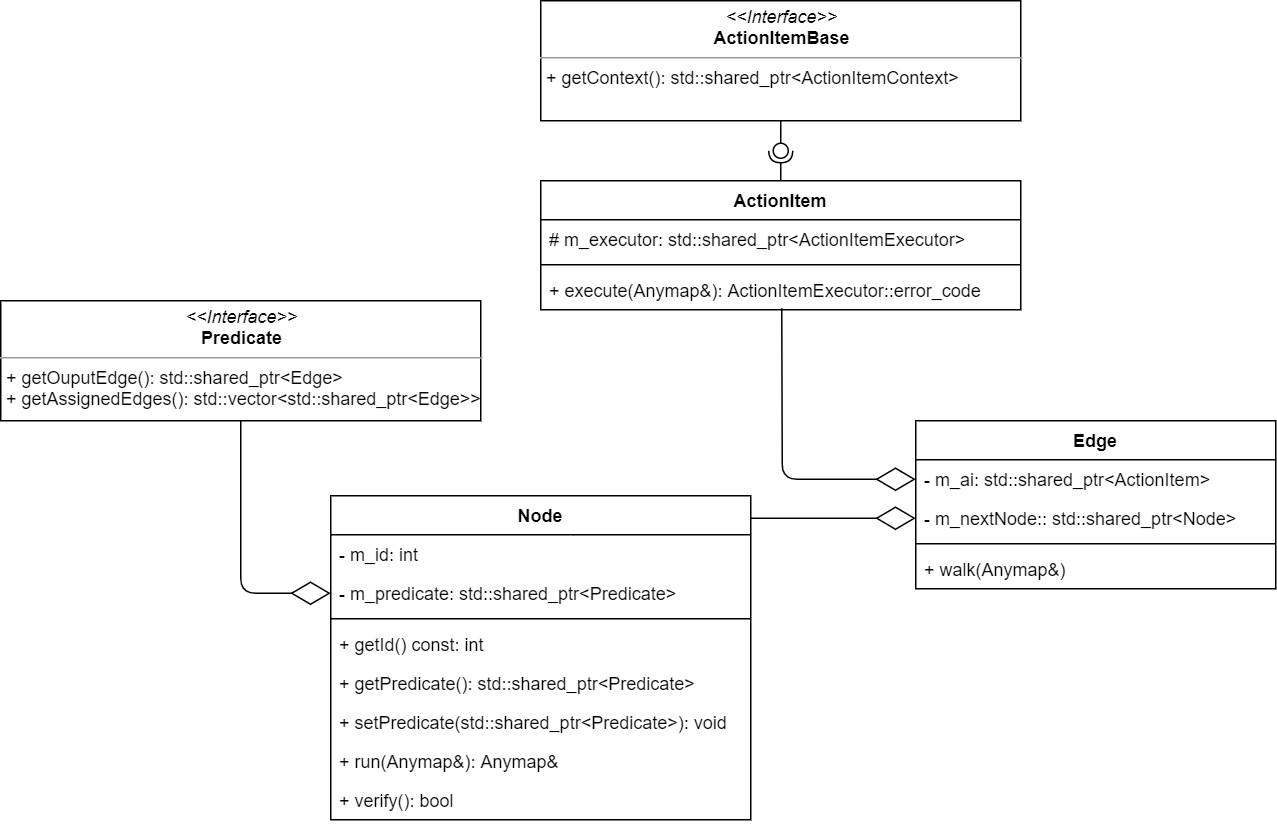
\includegraphics[width=\textwidth]{ResearchNotes/rndhpc_not_blo_2022_03_09/structure.png}
    \caption{Текущая структура классов, связанная с графовыми моделями в comsdk}\label{fig:oldGraphStructure}
\end{figure}

В существующей структуре классов можно выделить следующие недостатки.
\begin{enumerate}
    \item Отсутствует класс графа, который обеспечивал бы удобный интерфейс графовым моделям.
    \item Отсутствует структура данных, обеспечивающая хранение узлов, относящихся к конкретной графовой модели (включая вложенные графовые модели)%.контейнер, который бы инкапсулировал все 
    \item Индекс узла графа задаётся пользователем при инициализации, что не гарантирует его уникальности.\messnote{Непотнятно! Что вы хотели бы сделать?}
    \item Отсутствует структура данных, обеспечивающая хранение рёбер, относящихся к конкретной графовой модели (включая вложенные графовые модели). %контейнер, который бы инкапсулировал все 
    \item Отсутствует объект, который бы описывал связи между узлами и рёбрами; вместо этого эти связи прописаны в самих узлах и рёбрах, что затрудняет операции с графовой моделью (преобразования и проч.).\messnote{Непотнятно! Прошу уточнить.}
    \item Функции-предикаты привязываются к узлам, а не к рёбрам, что не соответствует требованиям синтаксических конструкций языка \gls{aDOT}.
    \item В текущей версии задачей функций-предикатов фактически является отбор рёбер, которые должны быть выполнены, а не проверка соответствия данных в узле определённому формату.
\end{enumerate}

%----------------------------------------------------------
% Атрибуты задачи
\noteattributes{}
%----------------------------------------------------------

%----------------------------------------------------------
\def\notedate{2022.03.23}
\def\currentauthor{Тришин~И.В., Соколов~А.П.}
%----------------------------------------------------------
\notestatement{rndhpcblo}{Требования к возможностям обхода графовых моделей в GBSE}

Графоориентированный подход \gls{gbse} подразумевает параллельное выполнение рёбер графа, выходящих из одной вершины. На рисунке \ref{fig:parallelExample} после выполнения функций перехода $F_{12}$ и~$F_{13}$, связанных с рёбрами, будет осуществлён переход в два независимых состояния данных $S_2$ и $S_3$ соответственно. Далее возникает задача правильным образом преобразовать данные из этих состояний в общее состояние $S_4$.

\begin{figure}[!ht]
    \centering
    \includegraphics[scale=0.3]{ResearchNotes/rndhpc_not_blo_2022_03_23/example.parallel.png}
    \caption{Пример графовой модели, предполагающей параллельное исполнение}
    \label{fig:parallelExample}
\end{figure}

\begin{remark}
Далее, допуская определённую нестрогость, говоря о том, что \uline{функции перехода, связываемые с рёбрами графовых моделей, выполняются в отдельных потоках выполнения}, будем считать, что они выполняются: либо в общем адресном пространстве текущего процесса выполнения, либо в разных процессах на одной или разных вычислительных системах. 

Другими словами, в рамках настоящей заметки не будем предполагать, что данные, формируемые в параллельных ветках графовой модели, размещаются в общей памяти.
\end{remark}

Рассматриваемый подход может способствовать значительному увеличению эффективности использования ресурсов вычислительной системы и, как следствие, ускорению процесса выполнения\footnote{В случае наличия доступных вычислительных ресурсов: нескольких ядер процессора.}, однако, предполагает необходимость реализации дополнительных второстепенных задач. Так для примера на рис.~\ref{fig:parallelExample} функции перехода $F_{12}$ и~$F_{13}$ должны выполняться параллельно (в двух разных потоках выполнения), а значит полученные в результате их выполнения данные, в общем случае\footnote{Речь идёт о самом общем случае, когда выпонение отдельных функций перехода допускается на разных вычислительных машинах или на кластерных системах с распределённой памятью.}, могут быть размещены в разных адресных пространствах разделённой оперативной памяти. Поэтому встаёт задача сбора этих данных в общую оперативную память при переходе в $S_4$. В момент разветвления графа должно (в общем случае) происходить \flqq разделение\frqq обрабатываемых данных, чтобы каждая ветвь работала со своим экземпляром данных. Помимо этого алгоритм обхода графовой модели должен корректно отрабатывать слияние ветвей графа.

\begin{figure}[!ht]
    \centering
    \includegraphics[scale=0.3]{ResearchNotes/rndhpc_not_blo_2022_03_23/example.parallel_then_linear.png}
    \caption{Пример графовой модели с совмещением ветвей}
    \label{fig:parallelThenLinearExample}
\end{figure}

На рисунке \ref{fig:parallelThenLinearExample} ветви $S_1 \rightarrow S_2 \rightarrow S_4$ и $S_1 \rightarrow S_3 \rightarrow S_4$ выполняются в разных потоках выполнения, но ребро $F_{45}$ должно быть выполнено только в одном потоке (если обратного не предполагает функция перехода этого ребра). Таким образом, очевидна необходимость в некоторой управляющей программной структуре, которая бы обеспечивала управление (запуск и завершение) различных потоков выполнения.

Кроме того, указанная управляющая программная структура должна поддерживать несколько вариантов параллельного исполнения. Среди прочих желательна поддержка:
\begin{enumerate}[label=\arabic*)]
    \item поочерёдного выполнения (в первую очередь для отладки);\messnote{Требуется пояснение! Использованы абстрактные обороты, например: поочерёдное выполнение, многопроцессное выполнение?}
    \item многопроцессного выполнения;\messnote{Требуется пояснение!}
    \item многопоточного выполнения;
    \item выполнения на удалённых узлах (через SSH-соединение).\messnote{Требуется пояснение!}
\end{enumerate}

Т.о. целесообразна поддержка единого интерфейса для различных режимов (стратегий) выполнения (параллельный, последовательный, распределённый и пр.) в рамках обозначенной управляющей программной структуры. % , разработчик мог создавать различные реализации этой структуры для каждого отдельного способа. 

%----------------------------------------------------------
% Атрибуты задачи
\noteattributes{}
%----------------------------------------------------------


%----------------------------------------------------------
\def\notedate{2022.04.13}
\def\currentauthor{Тришин И.В. (РК6-81Б)}
%----------------------------------------------------------
\notestatement{rndhpcblo}{Дополнительный обзор литературы и наброски для введения}
Методы решения задач, возникающие в процессе современных научно-технических исследований, зачастую предполагают выполнение большого количества операций обработки данных. Каждой такой операции требуются входные данные. По завершении выполнения операции получаются выходные данные. При этом выходные данные одной операции могут являться входными для одной или нескольких других операций. Между ними формируются зависимости по входным и выходным данным. Для учёта этих зависимостей возникает необходимость правильным образом организовать выполнение операций в пределах отдельно взятого метода и, в частности, при разработке программного обеспечения (ПО), которое реализовало бы данный метод. 

В наши дни популярность приобретает применение научных систем организации рабочего процесса (англ. scientific workflow systems). Такие системы позвояют автоматизировать процессы решения научно-технических задач, предоставляя средства организации и управления вычислительными процессами~\cite{DeelmanWorkflow2009}. Процесс работы с подобными системами состоит из 4 основных этапов:
\begin{enumerate}
    \item составление описания операций обработки данных и зависимостей между ними;
    \item распределение процессов обработки данных по вычислительным ресурсам;
    \item выполнение обработки данных;
    \item сбор и анализ результатов и статистики.
\end{enumerate}

Одной из ключевых особенностей подобного подхода к реализации методов решения научно-технических задач является выделение операций обработки данных в отдельные программные модули (функции, подпрограммы). При известных входных и выходных данных каждого модуля становится возможной их независимая разработка\cite{DanilovPar2011}. Это позволяет распределить их разработку между членами команды исследователей. Вследствие этого уменьшается объём работы по написанию исходных кодов, приходящийся на одного исследователя. Это в свою очередь облегчает отладку и написание документации, что положительно сказывается на общем качестве реализуемого ПО. Кроме того, 
%----------------------------------------------------------
\def\notedate{2022.05.17}
\def\currentauthor{Тришин И.В., Соколов А.П.}
%----------------------------------------------------------
\notestatement{rndhpcblo}{Современные форматы описания иерархических структур данных}

При выполнении курсового проекта по дисциплине \flqq Технологии Интернет\frqq\xspace была поставлена задача разработать программный инструмент описания\pdfcomment{Скорее речь об инструменте визуализации...} структуры состояния данных вычислительных методов~\cite{SokolovPershin2018}. Данный инструмент планируется в дальнейшем встроить как компонент в средство визуализации состояний данных. Разработка данного средства направлена на повышение прозрачности и наглядности взаимодействия с программным инструментарием \gls{gbse}.

Кроме того, разработка инструмента описания состояний данных направлена на поддержание идеи документирования алгоритмов и вычислительных методов, реализуемых по методологии GBSE.

%-------------------
\subsubsection{Описание структуры состояния данных}

Т.н. <<состояние данных>>\cite{SokolovPershin2018} представляет собой множество именованных переменных фиксированного типа, характерное для конкретного этапа вычислительного метода или алгоритма. Данные в соответствующем состоянии, как правило, удобно хранить в виде ассоциативного массива. Тип отдельной переменной может быть как скалярным (целое, логическое, вещественное с плавающей запятой и пр.), так и сложным <<векторным>> (структурой, классом, массивом и пр.). Примером сложного <<векторного>> типа является, в свою очередь, ассоциативный массив со строковыми ключами, при этом конкретная переменная этого типа будет хранить, как правило, адрес этого массива. В общем случае элементы данного массива могут иметь разные типы. 

%Достоиством использования таких ассоциативных массивов является возможность группировки данных.
В рассматриваемом случае возникает возможность организации хранения состояния данных в виде иерархических структур.

%Помимо этого, поскольку каждый элемент ассоциативного массива обладает ключом, типом и значением, что повторяет общую структуру элемента состояния данных, возникает возможность организовать состояния данных в виде иерархических структур.

Таким образом, для описания состояний данных требуется формат, который бы поддерживал гетерогенные (т.е. разнотипные) иерархические структуры данных.

%-------------------
\subsubsection{Анализ известных форматов}

Одними из первых рассмотренных были форматы для хранения научных данных HDF4 и HDF5~\cite{HDFOffCite}. Данные бинарные форматы позволяют хранить большие объёмы гетерогенной информации и поддерживают иерархическое представление данных. В нём используется понятие набора данных (англ. dataset), которые объединяются в группы (англ. group). Кроме того, формат HDF5 считается <<самодокументирующимся>>, поскольку каждый его элемент -- набор данных или их группа -- имеет возможность хранить метаданные, служащие для описания содержимого элемента. Существует официальный API данного формата для языка С++ с открытым исходным кодом. Одним из гланвых недостатков HDF5 является необходимость дополнительного ПО для просмотра и редактирования данных в этом формате, поскольку он является бинарным.

Альтернативой бинарным форматам описания данных являются текстовые. Среди них были рассмотрены форматы XML (Extensible Markup Language) и JSON (Javascript Object Notation). Главным преимуществом формата XML является его ориентированность на древовидные структуры данных и лёгкость лексико-синтаксического разбора файлов этого формата. Среди недостатков стоит выделить потребность в сравнительно большом количестве вспомогательных синтаксических конструкций, необходимых для структурирования (тегов, атрибутов). Они затрудняют восприятие чистых данных и увеличивают итоговый объём файла. 

Формат JSON, так же, как и XML рассчитан на иерархические структуры данных, но является не столь синтаксически нагруженным, что облегчает восприятие информации человеком~\cite{JSONvsXML}. Кроме того, крайне важным преимуществом JSON является его поддержка по-умолчанию средствами языкы программирования Javascript, который используется при разработке веб-приложений. При этом JSON также обладает рядом недостатков. Среди них сниженная, по сравнению с XML надёжность, отсутствие встроенных средств валидации и отсутствие поддержки пространств имён, что снижает его расширяемость.


%----------------------------------------------------------
% Атрибуты задачи
\noteattributes{}
%----------------------------------------------------------


%\input{ResearchNotes/rndhpc_not_edt_@year@_@month@_@id@.tex}

\section{\rndprojectdscr{rndhpcrpc}}

%----------------------------------------------------------
\def\notedate{2022.06.17}
\def\currentauthor{Амелькина А.-М. (РК6)}
%----------------------------------------------------------
\notestatement{rndhpcrpc}{Удаленный запуск кода Waleffe_flow.Fortran}
%----------------------------------------------------------

\subsubsection{Описание структуры программы Waleffe_flow.Fortran}
Структура директорий исходных кодов и запусков программы Waleffe\_flow.Fortran изображена на рисунке \ref{structure}.
\begin{figure}[!ht]
	\centering
	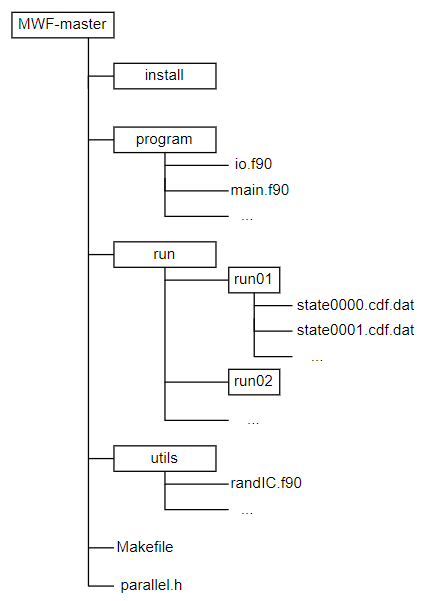
\includegraphics[width=0.45\textwidth]{ResearchNotes/rndcmp_not_rcs_2022_06_17/MWF-иерархия.png}
	\caption{Структура программы Waleffe\_flow.Fortran}\label{structure}
\end{figure} 

%----------------------------------------------------------
\subsubsection{Удаленный запуск кода}

Для подключения к удаленной машине используется SSH -- сетевой протокол прикладного уровня, позволяющий производить удалённое управление операционной системой и туннелирование TCP-соединений  \cite{ssh}.

Для запуска программы Waleffe\_flow.Fortran на удаленной машине необходимо выполнить следующие команды:
\begin{enumerate}
    \item Подключение к удаленной машине \cite{ssh-comand}:
            \begin{verbatim}
            ssh user@server  \end{verbatim}
        В данной работе использовалась виртуальная машина с именем hpc.rk6.bmstu.ru и пользователь amamelkina, поэтому команда выглядела следующим образом: \begin{verbatim}
            ssh amamelkina@hpc.rk6.bmstu.ru   \end{verbatim}
    \item Переход в директорию с программой  \cite{ubuntu-comand}:
            \begin{verbatim}
            cd /home/amamelkina/MWF-master    \end{verbatim}
    \item Чтобы настроить среду для использования библиотек MPI, нужно загрузить соответствующий модуль окружающей среды:
            \begin{verbatim}
            module load mpi \end{verbatim}
    \item Сборка:
            \begin{verbatim}
            make
            make install    \end{verbatim}
    \item Создание начальных условий: \label{IC}
            \begin{verbatim}
            make util
            ./randIC.out    \end{verbatim}
    \item Далее необходимо создать папку, в которую будут записываться результаты. Такие наборы результатов хранятся в папке run. В папке run создается папка с номером (например run10), в нее копируются файлы /install/main.info, /install/main.out. Файл state0000.cdf.dat, полученный в результате выполнения пункта \ref{IC}, должен быть переименован в state.cdf.in и тоже скопирован в новую папку результатов.
    \item Затем нужно перейти в созданную папку и запустить программу:
            \begin{verbatim}
            ./main.out    \end{verbatim}
    \item После остановки программы, когда будет получено необходимое количество данных, можно отключаться от удаленной машины с помощью команды:
            \begin{verbatim} 
            exit \end{verbatim}
    \item Последний шаг -- скопировать результат с удаленной машины на локальную \cite{ssh-cp}:
            \begin{verbatim}
            scp -r user@server:<адрес/откуда/копируем>
                               <адрес/куда/копируем>  \end{verbatim}
\end{enumerate}

Видно, что запуск данной программы на удаленной машине требует выполнения множества команд. Упростим запуск до одной команды -- запуска python-скрипта, в котором будет реализован процесс удаленного запуска.

%----------------------------------------------------------
\subsubsection{Программная реализация}

Для реализации необходимого python-скрипта была использована библиотека fabric. Fabric – это библиотека Python и инструмент командной строки для оптимизации использования SSH для развертывания приложений или задач системного администрирования \cite{fabric-doc}.

Для работы с fabric первым делом нужно создать fabfile и разместить в структуре файлов так, как показано на рисунке \ref{structure_fab}.
\begin{figure}[!ht]
	\centering
	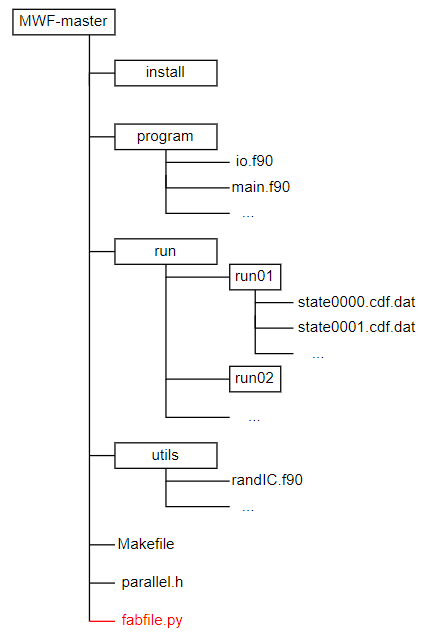
\includegraphics[width=0.45\textwidth]{ResearchNotes/rndcmp_not_rcs_2022_06_17/MWF-иерархия_fab.png}
	\caption{Размещение fabfile}\label{structure_fab}
\end{figure} 

Fabfile -- это то, что контролирует то, что выполняет fabric. Он называется fabfile.py и запускается командой fab. Все функции, определенные в этом файле, будут отображаться как подкоманды fab. Они выполняются на одном или нескольких серверах. Эти серверы могут быть определены либо в fabfile, либо в командной строке \cite{fabric-fab}.

Добавим сервер в fabfile, определив его в переменной окружения env (листинг \ref{host}) \cite{fabric-env}. 
\begin{lstlisting}[label=host, language=Python, caption=Добавление сервера в переменную окружения env] 
        env.hosts = ['hpc.rk6.bmstu.ru']
\end{lstlisting}

Fabric по умолчанию использует локальное имя пользователя при подключении SSH, но при необходимости его можно переопределить, используя env.user. Предоставим пользователю программы возможность ввести имя (листинг \ref{user}). Это реализовано с помощью функции prompt(text, default='', ...) \cite{fabric-func}.
Данная функция выдаёт пользователю запрос с текстом text и возвращает полученное значение. Для удобства к text будет добавлен одиночный пробел.
Если передан параметр default, то он будет выведен в квадратных скобках и будет использоваться в случае, если пользователь ничего не введёт (т.e. нажмёт Enter без ввода текста). По умолчанию значением default является пустая строка.
\begin{lstlisting}[label=user, language=Python, caption=Добавление имени пользователя в переменную окружения env] 
        user = prompt("Enter username", default=’amamelkina’)
        env.user = user
\end{lstlisting}

Также пользователю нужно ввести время в секундах, в течение которого будет выполняться программа.

Затем с помощью функции run(command, ...), которая запускает команду оболочки на удалённом узле, выполняется запуск программы Waleffe\_flow.Fortran.

Также используются функции put(local\_path=None, remote\_path=None, ...) и get(remote\_path, local\_path = None) для загрузки файлов на удаленный сервер и скачивания файлов с удалённого сервера соответственно.

Листинг кода python-скрипта представлен в Приложении.

Для запуска fabric предоставляет команду fab, которая считывает свою конфигурацию из файла fabfile.py.

В листинге \ref{hello} представлена простая функция, с помощью которой будет продемонстрировано, как использовать fabric \cite{fabric-hello}. Эта функция сохранена как fabfile.py в текущем рабочем каталоге.
\begin{lstlisting}[label=hello, language=Python, caption=Пример функции]
        def hello():
            print("Hello!")
\end{lstlisting}

 Функция приветствия может быть выполнена с помощью fab инструмента следующим образом:
\begin{verbatim}
        fab hello
\end{verbatim}

В результате выполнения этой команды будет выведено "Hello!".

Таким образом, для запуска программы Waleffe\_flow.Fortran на удаленной машине теперь необходимо выполнить только одну команду:
\begin{verbatim}
        fab run_fortran
\end{verbatim}

В результате работы данного python-скрипта на персональном компьютере в папке run появится новая папка с результатами запуска.

%----------------------------------------------------------
% Атрибуты задачи
\noteattributes{}
%----------------------------------------------------------

%----------------------------------------------------------

%----------------------------------------------------------
\renewcommand\bibname{\small{Литература}}\label{bibs}
\bibliographystyle{utf8gost705u}
\bibliography{bibliography,bibliography-avtoreferat}
%----------------------------------------------------------
\end{document}
%----------------------------------------------------------



